\chapter{Documentos}\label{cap:documentos}

Todos los documentos viven dentro de un expediente. Antes de cualquier tarea
de este capítulo, abra el expediente (\cref{sec:buscar-expediente}) y haga
clic en la pestaña \textbf{Documentos}.

\begin{table}[H]
  \centering
  \caption{Qué puede hacer cada rol con los documentos.}\label{tab:permisos-documentos}
  \begin{tabularx}{\textwidth}{Y C{1.4cm} C{1.4cm} C{1.4cm}}
    \toprule
    \textbf{Acción} & \textbf{Adm.} & \textbf{Litig.} & \textbf{Asist.} \\
    \midrule
    Consultar, subir, clasificar y agregar versiones & Sí & Sí & Sí \\
    Descargar el archivo, verificar y descargar evidencia & Sí & Sí & Sí \\
    Sellar documento & Sí & Sí & No \\
    Crear contrato con el Cliente & Sí & Sí & No \\
    Firmar personalmente & No & Sí & No \\
    \bottomrule
  \end{tabularx}
\end{table}

El Litigante y el Asistente legal solo ven los documentos de sus expedientes
asignados.

% ---------------------------------------------------------------------
\section{Consultar los documentos del expediente}\label{sec:consultar-documentos}

\paraque Localiza un documento del expediente y muestra en qué estado se
encuentra.

\disponible Administrador, Litigante y Asistente legal.

\pasos
\begin{enumerate}
  \item En la pestaña \textbf{Documentos}, revise el \textbf{Archivo documental}.
  \item Para buscar, escriba parte del nombre en \textbf{Buscar por nombre...}
        y haga clic en \textbf{Buscar}.
  \item Para filtrar por estado, elija \textbf{Todos los estados},
        \textbf{Pendientes de sello} o \textbf{Sellados}.
  \item Para filtrar por clasificación, abra \textbf{Filtros de clasificación},
        llene \textbf{Tipo exacto}, \textbf{Clasificación exacta} o
        \textbf{Etiqueta exacta} y haga clic en \textbf{Aplicar filtros}.
  \item Haga clic en \textbf{Abrir} junto al documento.
\end{enumerate}

\begin{figure}[H]
  \centering
  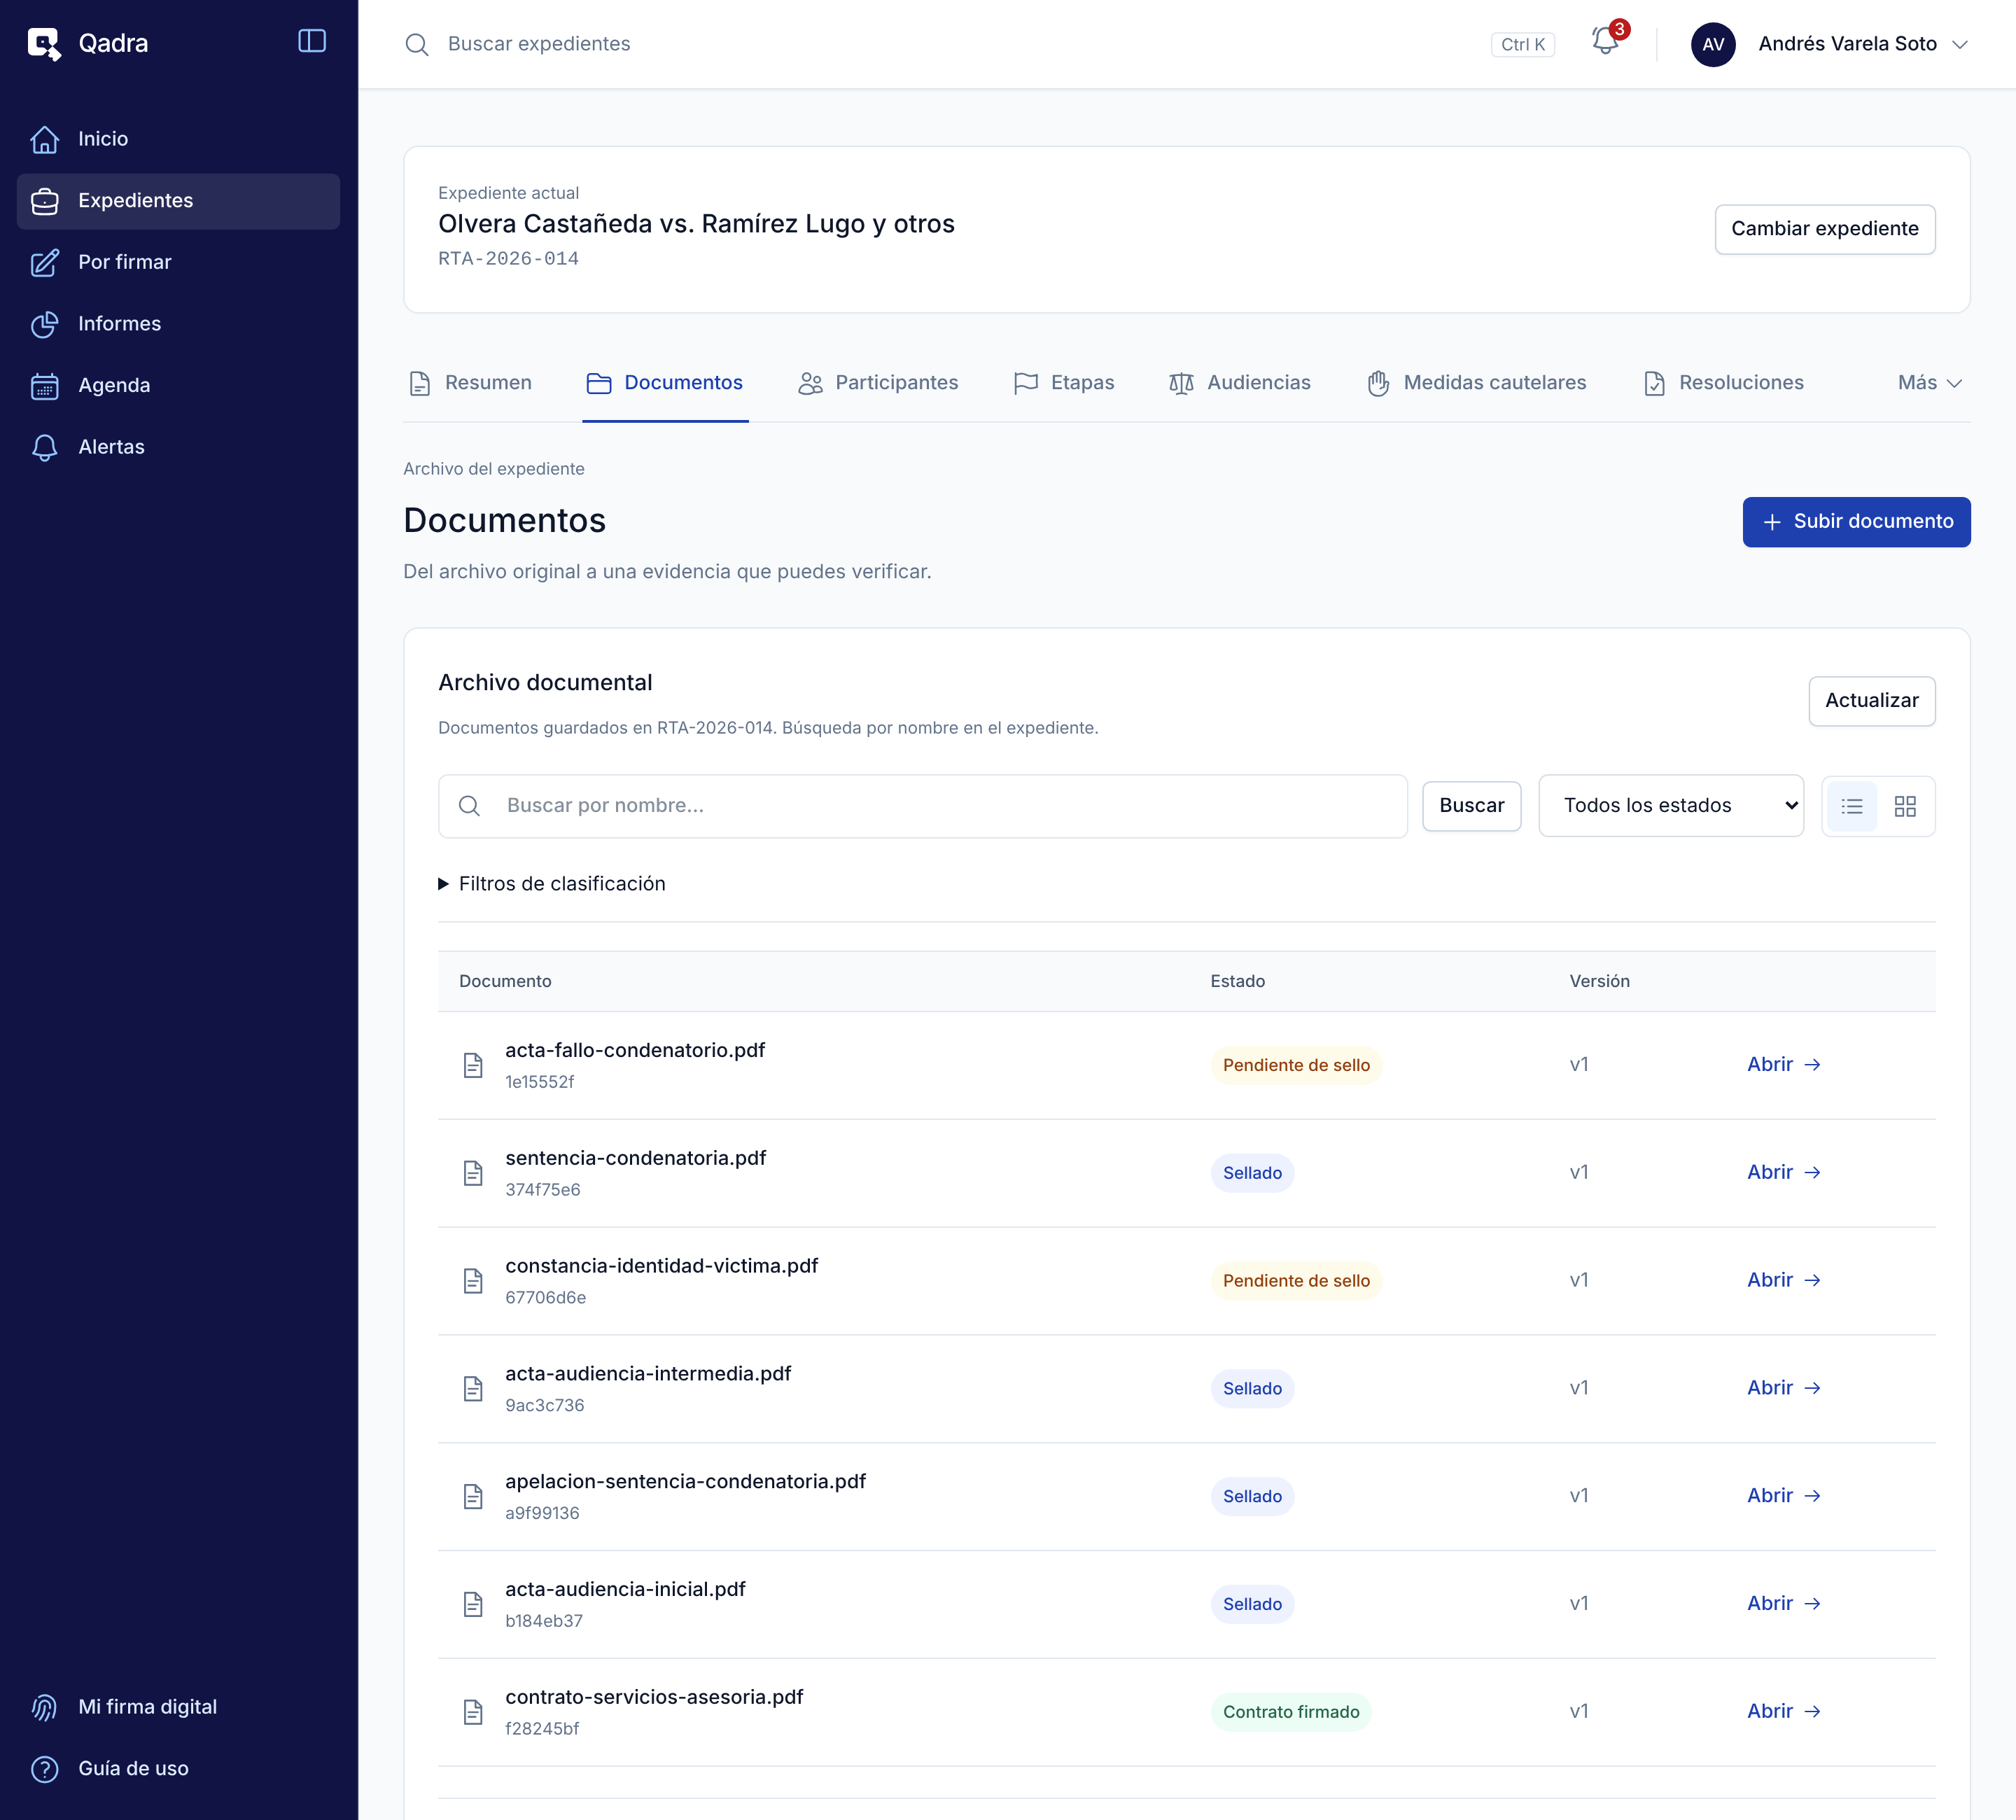
\includegraphics[width=0.9\textwidth]{capturas/A-18-archivo-documental.png}
  \caption{Archivo documental del expediente.}
  \label{fig:manual-archivo-documental}
\end{figure}

\resultado Se abre la \textbf{Ficha documental} del documento
(\cref{sec:ficha-documental}).

\begin{table}[H]
  \centering
  \caption{Estados de un documento en la lista.}\label{tab:estados-documento}
  \begin{tabularx}{\textwidth}{L{3.6cm} Y}
    \toprule
    \textbf{Estado} & \textbf{Qué significa} \\
    \midrule
    \textbf{Pendiente de sello} & El archivo está guardado, pero aún no tiene sello. \\
    \textbf{Sellado}            & Tiene firma y sello de tiempo; ya puede verificarse. \\
    \textbf{Verificado}         & La última verificación pasó todas las comprobaciones. \\
    \textbf{Revisar evidencia}  & La última verificación encontró un problema
                                  (\cref{sec:verificar-documento}). \\
    \textbf{En contrato}        & La versión está en firma con el Cliente. \\
    \textbf{Contrato firmado}   & El Cliente y el despacho firmaron la versión. \\
    \bottomrule
  \end{tabularx}
\end{table}

\nota{Los filtros de clasificación buscan el valor completo y distinguen
mayúsculas y acentos. Para quitarlos, haga clic en \textbf{Limpiar filtros}.}

% ---------------------------------------------------------------------
\section{Subir un documento}\label{sec:subir-documento}

\paraque Agrega un archivo al expediente y lo guarda cifrado como su
versión 1.

\disponible Administrador, Litigante y Asistente legal. El expediente debe
estar activo.

\pasos
\begin{enumerate}
  \item En la pestaña \textbf{Documentos}, haga clic en
        \textbf{Subir documento}.
  \item Arrastre su archivo a la zona \textbf{Arrastra tu archivo aquí}, o
        haga clic en ella para seleccionarlo desde su equipo.
  \item Revise el \textbf{Nombre del documento} que Qadra sugiere. Puede
        cambiarlo usando solo letras sin acentos, números, puntos, guiones o
        guiones bajos (hasta 124 caracteres).
  \item Si lo desea, indique el \textbf{Tipo de documento (opcional)}, la
        \textbf{Clasificación (opcional)} y sus etiquetas
        (\cref{sec:clasificar-documento}).
  \item Haga clic en \textbf{Cargar documento}.
\end{enumerate}

\begin{figure}[H]
  \centering
  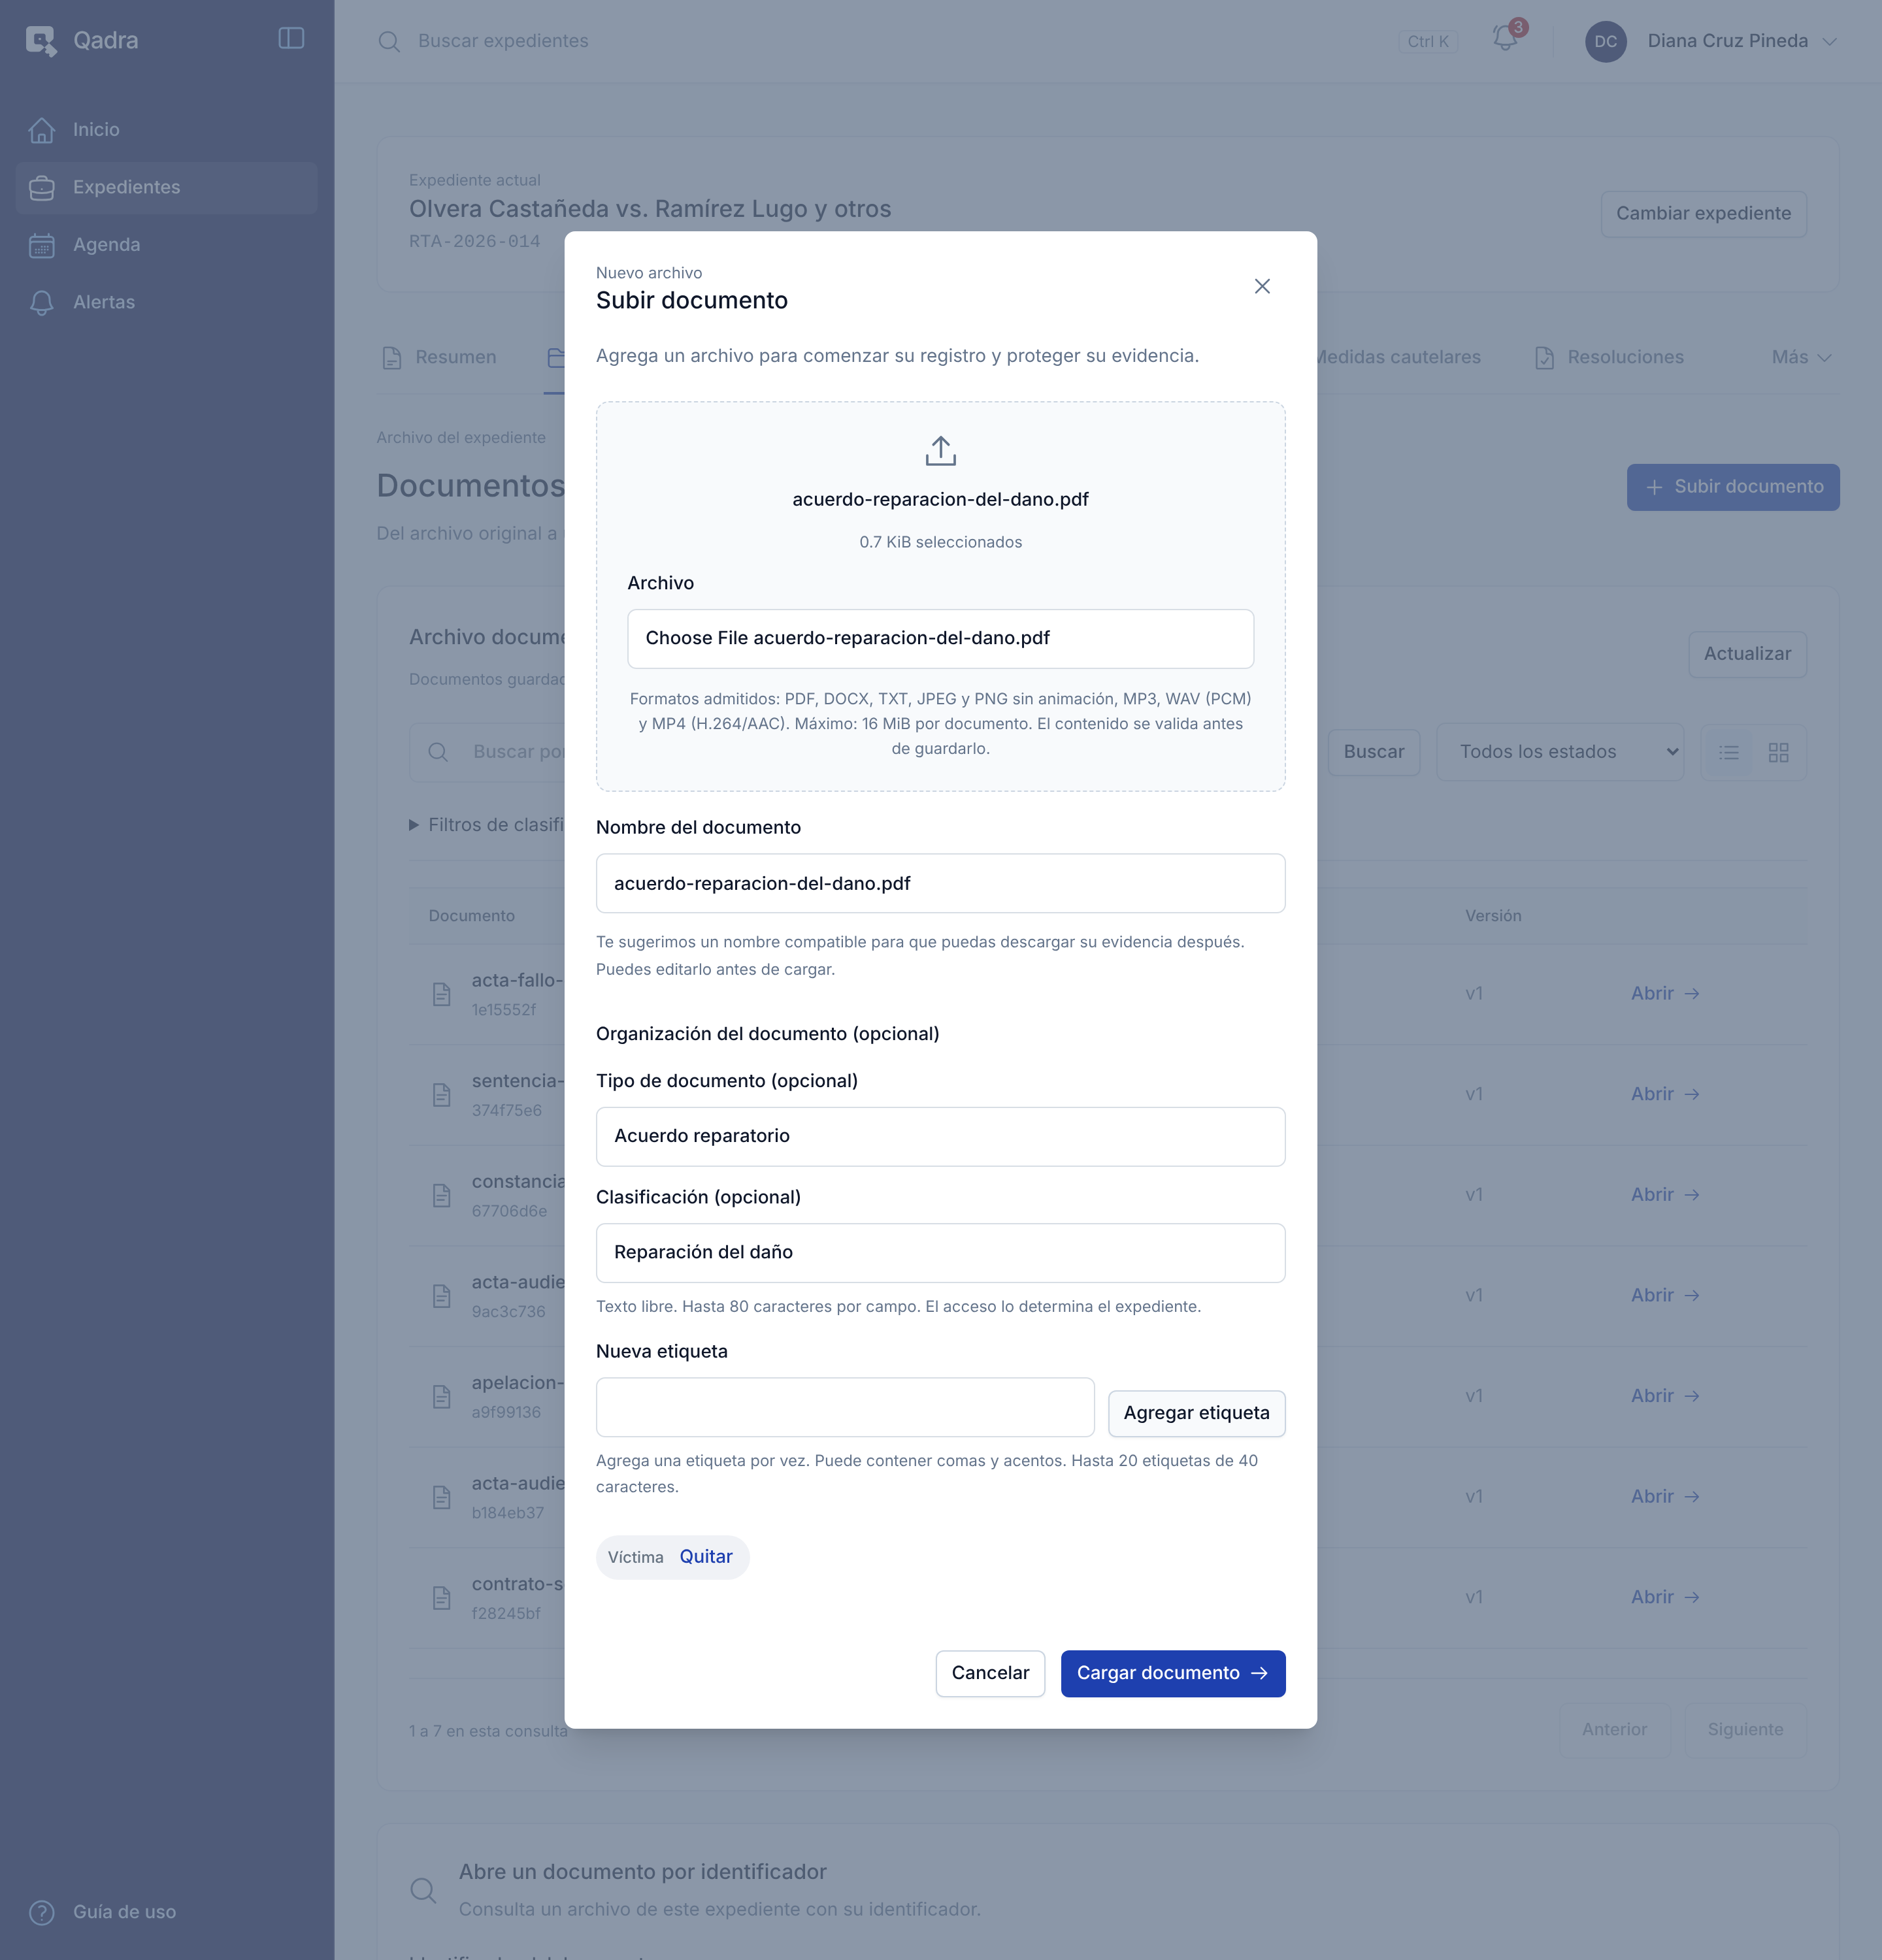
\includegraphics[width=0.9\textwidth]{capturas/A-19-subir-documento.png}
  \caption{Carga de un documento.}
  \label{fig:manual-subir-documento}
\end{figure}

\resultado El documento aparece en el archivo como
\textbf{Pendiente de sello}, en su versión 1.

\begin{table}[H]
  \centering
  \caption{Archivos admitidos.}\label{tab:formatos}
  \begin{tabularx}{\textwidth}{L{3.6cm} Y}
    \toprule
    \textbf{Concepto} & \textbf{Regla} \\
    \midrule
    Formatos & PDF, DOCX, TXT, JPEG y PNG sin animación, MP3, WAV (PCM) y
               MP4 (H.264/AAC). \\
    Tamaño máximo & 16 MiB por documento. \\
    Validación & Qadra revisa el contenido antes de guardarlo. Un archivo
                 dañado o de otro formato se rechaza. \\
    \bottomrule
  \end{tabularx}
\end{table}

\begin{itemize}
  \item Si el archivo es demasiado grande: \enquote{El archivo supera el
        límite de 16 MiB.}
  \item Si el formato no se admite: \enquote{El formato del archivo no está
        admitido. Elige un archivo de un formato compatible.}
  \item Si la carga se interrumpe, aparece \enquote{No se pudo confirmar la
        carga anterior.} Haga clic en \textbf{Consultar documentos actuales}
        antes de cargarlo otra vez, para no duplicarlo.
\end{itemize}

% ---------------------------------------------------------------------
\section{Ficha de un documento}\label{sec:ficha-documental}

\paraque Reúne el estado, las acciones, la clasificación y las versiones de
un documento.

\disponible Administrador, Litigante y Asistente legal.

La \textbf{Ficha documental} tiene, de arriba hacia abajo:
\begin{itemize}
  \item \textbf{Acciones:} \textbf{Descargar archivo},
        \textbf{Sellar documento}, \textbf{Verificar integridad},
        \textbf{Descargar evidencia} y, según el rol, \textbf{Crear contrato}
        o \textbf{Firmar personalmente}.
  \item \textbf{Pestañas:} \textbf{Resumen} (el recorrido del documento),
        \textbf{Verificación} (el resultado de la última verificación) y
        \textbf{Evidencia} (el paquete ZIP).
  \item \textbf{Clasificación actual del documento}
        (\cref{sec:clasificar-documento}).
  \item \textbf{Versiones de contenido} (\cref{sec:agregar-version}).
\end{itemize}

\begin{figure}[H]
  \centering
  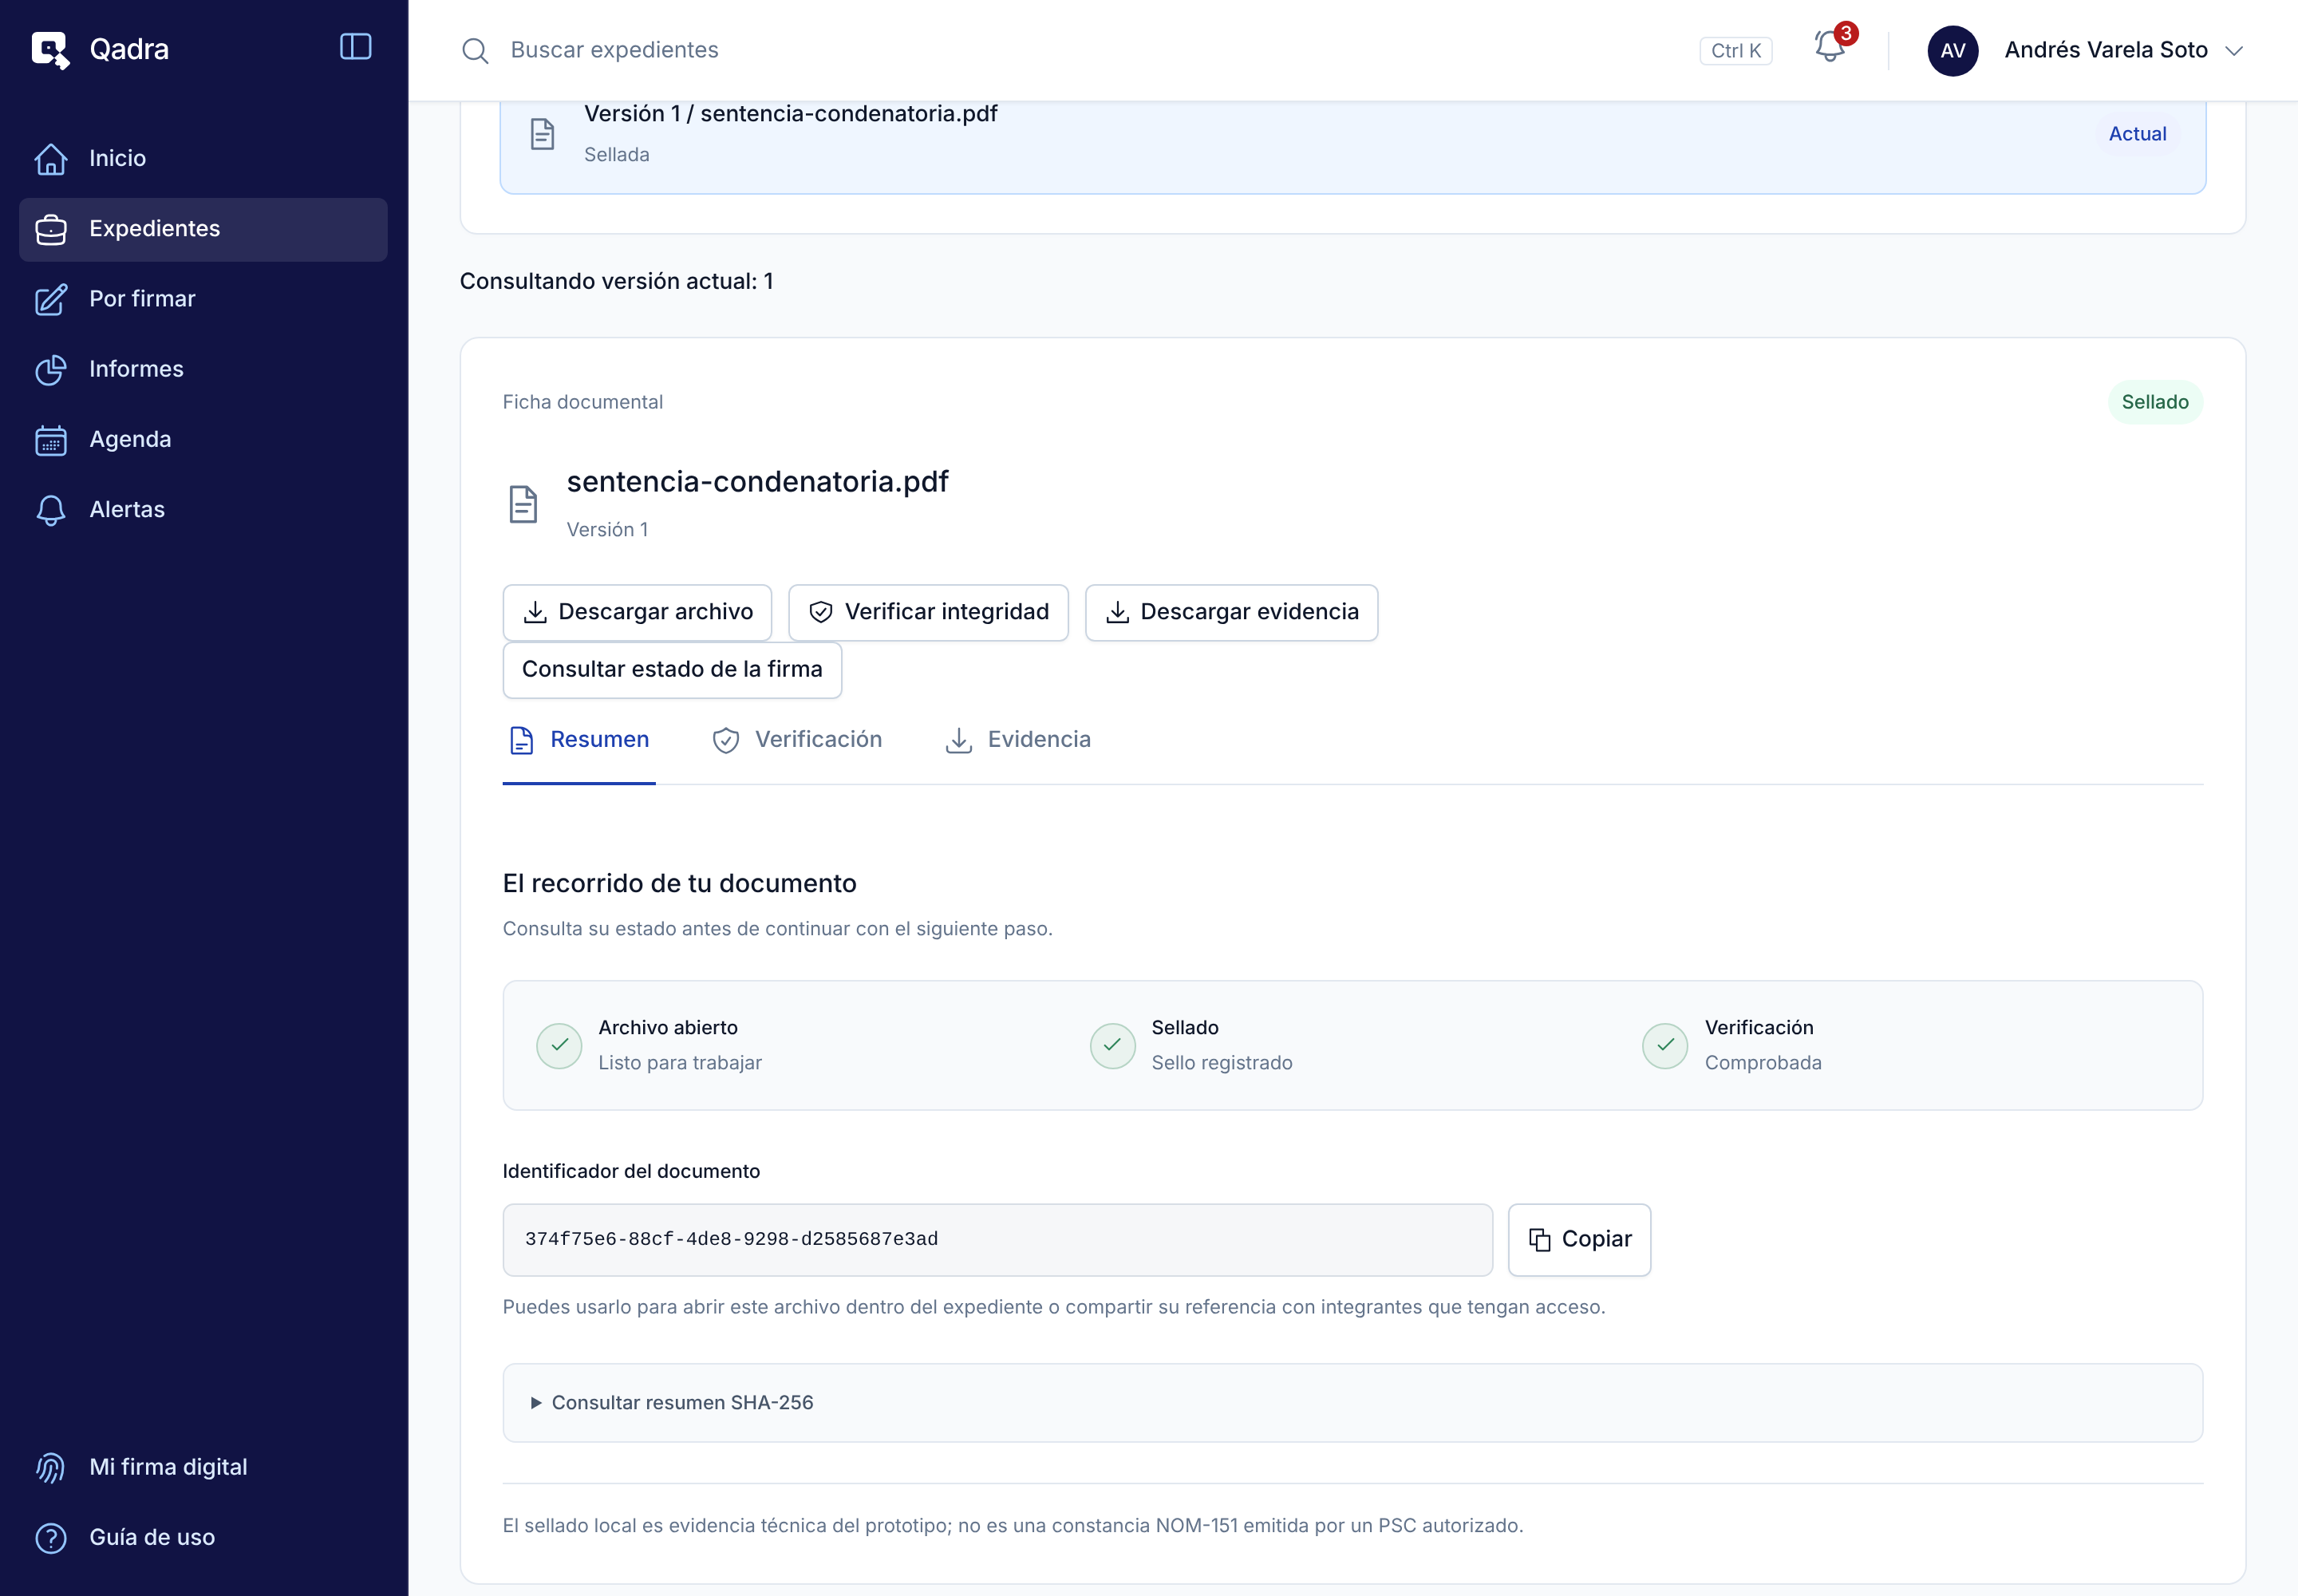
\includegraphics[width=0.9\textwidth]{capturas/A-20-ficha-documental.png}
  \caption{Ficha documental.}
  \label{fig:manual-ficha-documental}
\end{figure}

\begin{itemize}
  \item \textbf{Descargar archivo} entrega el archivo original de la versión
        elegida, después de comprobar que no cambió.
  \item En la pestaña \textbf{Resumen}, el botón \textbf{Copiar} copia el
        \textbf{Identificador del documento} para compartirlo con integrantes
        que tengan acceso.
\end{itemize}

% ---------------------------------------------------------------------
\section{Clasificar y etiquetar un documento}\label{sec:clasificar-documento}

\paraque Organiza el documento por tipo, clasificación y etiquetas para
encontrarlo después.

\disponible Administrador, Litigante y Asistente legal.

\pasos
\begin{enumerate}
  \item En la ficha del documento, busque
        \textbf{Clasificación actual del documento} y haga clic en
        \textbf{Editar clasificación}.
  \item Escriba el \textbf{Tipo de documento (opcional)} y la
        \textbf{Clasificación (opcional)}, de hasta 80 caracteres cada uno.
  \item Escriba una etiqueta en \textbf{Nueva etiqueta} y haga clic en
        \textbf{Agregar etiqueta}. Repita para cada etiqueta (hasta 20, de
        40 caracteres).
  \item Haga clic en \textbf{Guardar clasificación}.
\end{enumerate}

\begin{figure}[H]
  \centering
  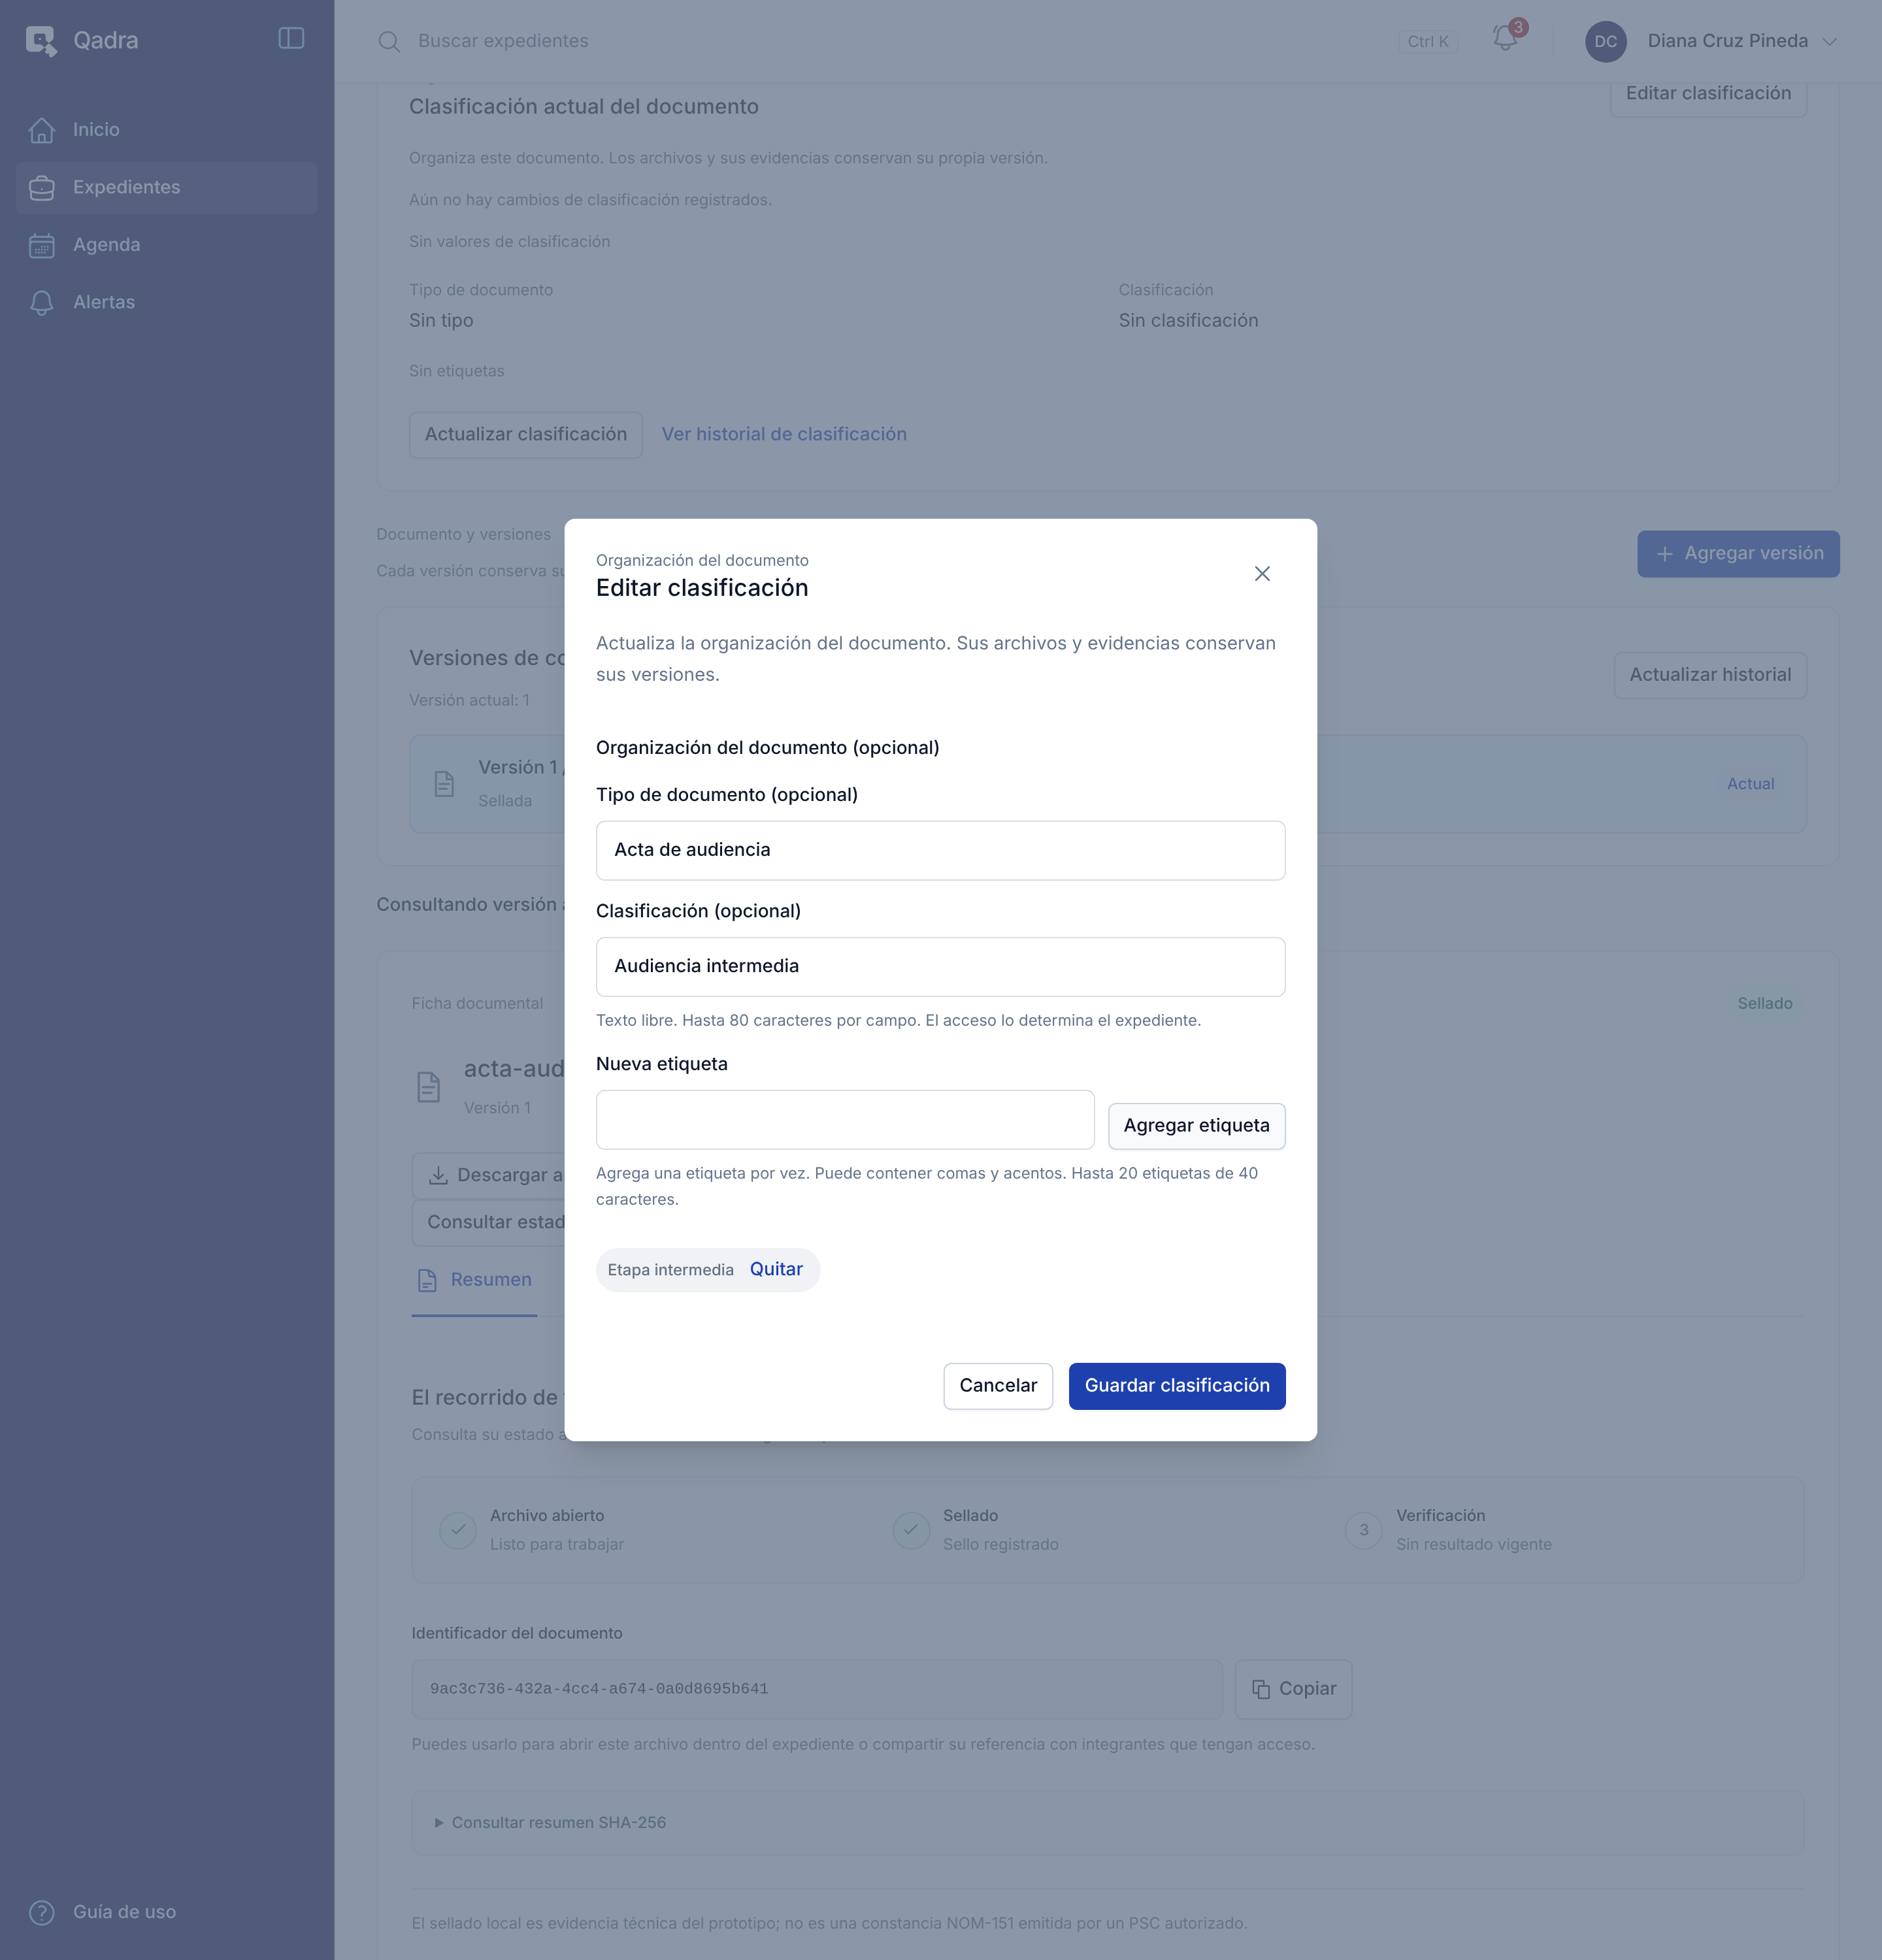
\includegraphics[width=0.9\textwidth]{capturas/A-21-editar-clasificacion.png}
  \caption{Clasificación de un documento.}
  \label{fig:manual-editar-clasificacion}
\end{figure}

\resultado La ficha muestra los valores nuevos. Para ver los cambios
anteriores, haga clic en \textbf{Ver historial de clasificación}.

\nota{Cambiar la clasificación no modifica el archivo, su firma ni su sello.
Si otra persona la cambió al mismo tiempo, Qadra le pide comparar los
valores actuales antes de guardar.}

% ---------------------------------------------------------------------
\section{Agregar una versión}\label{sec:agregar-version}

\paraque Guarda un archivo actualizado en el mismo documento sin borrar las
versiones anteriores ni su evidencia.

\disponible Administrador, Litigante y Asistente legal. El expediente debe
estar activo.

\pasos
\begin{enumerate}
  \item En la ficha del documento, haga clic en \textbf{Agregar versión}.
  \item Seleccione o arrastre el archivo en
        \textbf{Archivo de la nueva versión}.
  \item Revise el \textbf{Nombre de la nueva versión}.
  \item Haga clic en \textbf{Guardar nueva versión}.
\end{enumerate}

\begin{figure}[H]
  \centering
  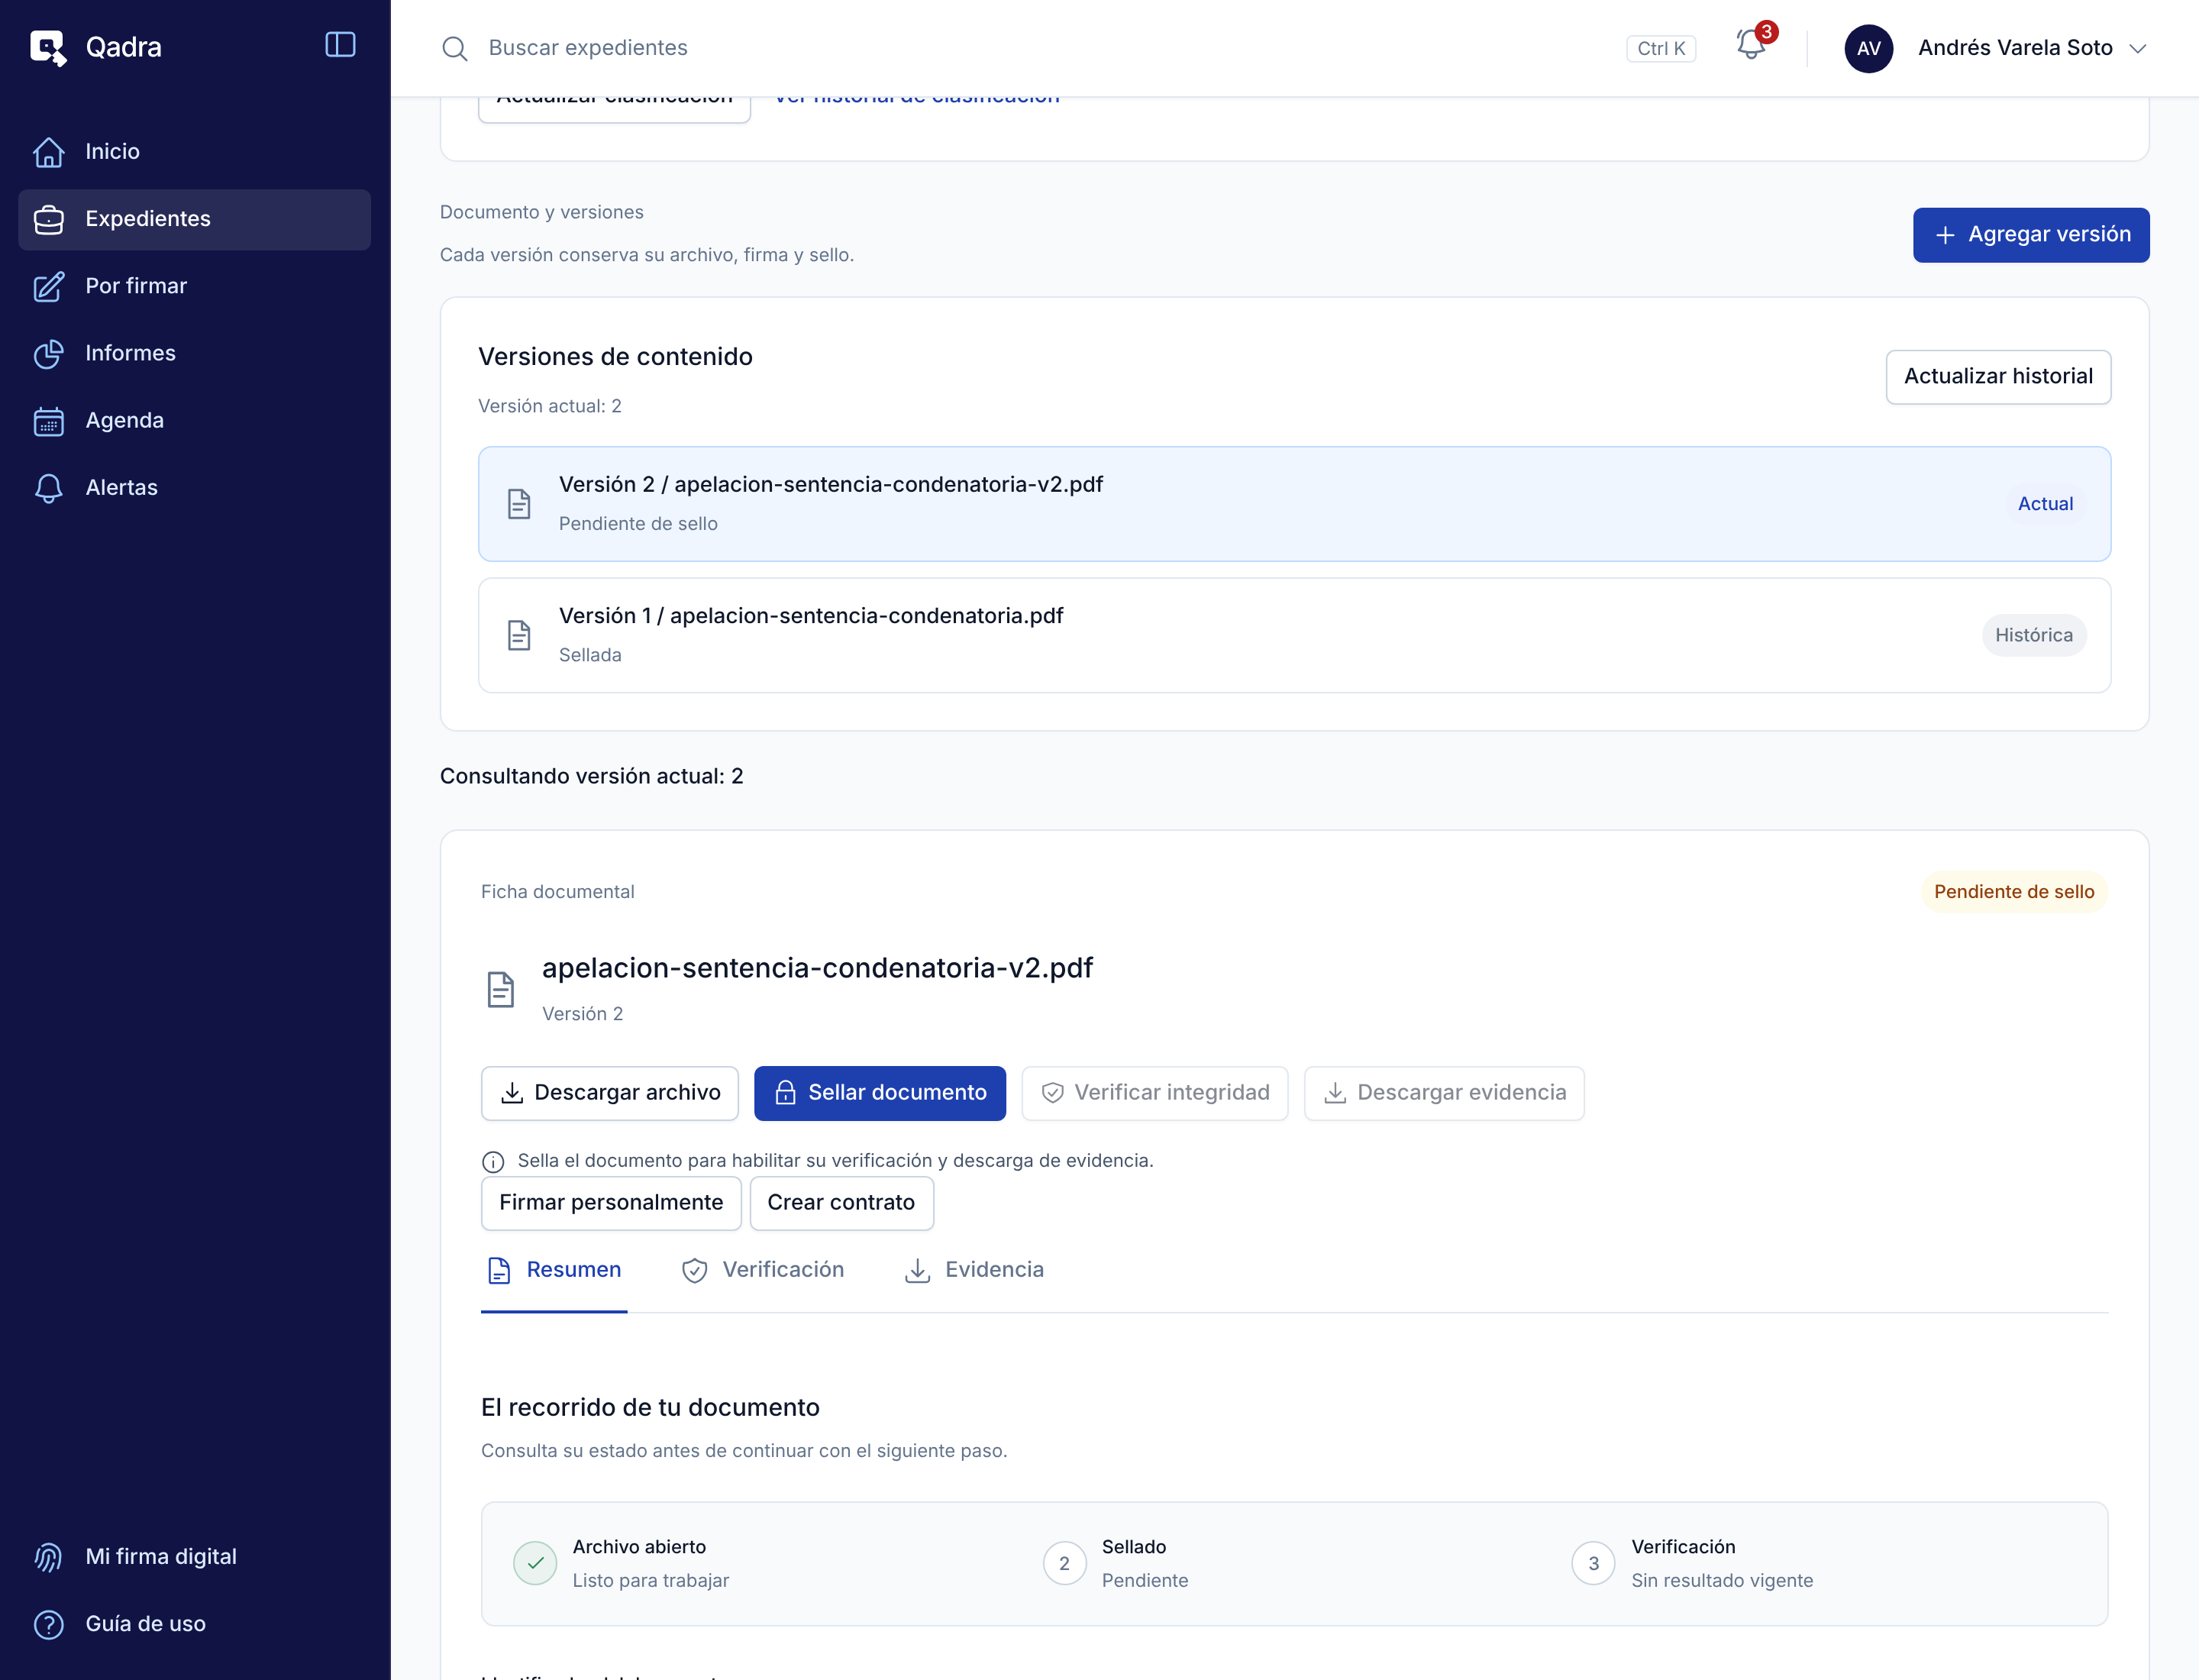
\includegraphics[width=0.9\textwidth]{capturas/A-22-versiones.png}
  \caption{Historial de versiones de un documento.}
  \label{fig:manual-versiones}
\end{figure}

\resultado La nueva versión aparece como \textbf{Actual} en
\textbf{Versiones de contenido}; las anteriores quedan como
\textbf{Histórica}.

\begin{itemize}
  \item Para trabajar con una versión anterior, haga clic en su fila. Las
        acciones de la ficha (descargar, sellar, verificar) se aplican a la
        versión elegida.
  \item Si otra persona agregó una versión mientras usted preparaba la suya,
        aparece \enquote{El documento cambió mientras preparabas el archivo.}
        Haga clic en \textbf{Consultar versión actual}, revise y confirme de
        nuevo. Su archivo se conserva.
\end{itemize}

% ---------------------------------------------------------------------
\section{Sellar un documento}\label{sec:sellar-documento}

\paraque Registra la firma del servidor y el sello de tiempo de la versión,
con su identidad. Después podrá verificarla y descargar su evidencia.

\disponible Administrador y Litigante. El expediente debe estar activo.

\importante{El sellado no se puede deshacer desde Qadra. Revise que la
versión elegida sea la correcta antes de confirmar.}

\pasos
\begin{enumerate}
  \item En la ficha del documento, elija la versión que desea sellar.
  \item Haga clic en \textbf{Sellar documento}.
  \item Lea el aviso \textbf{¿Registrar el sello del servidor?} y haga clic
        en \textbf{Confirmar sellado}.
\end{enumerate}

\begin{figure}[H]
  \centering
  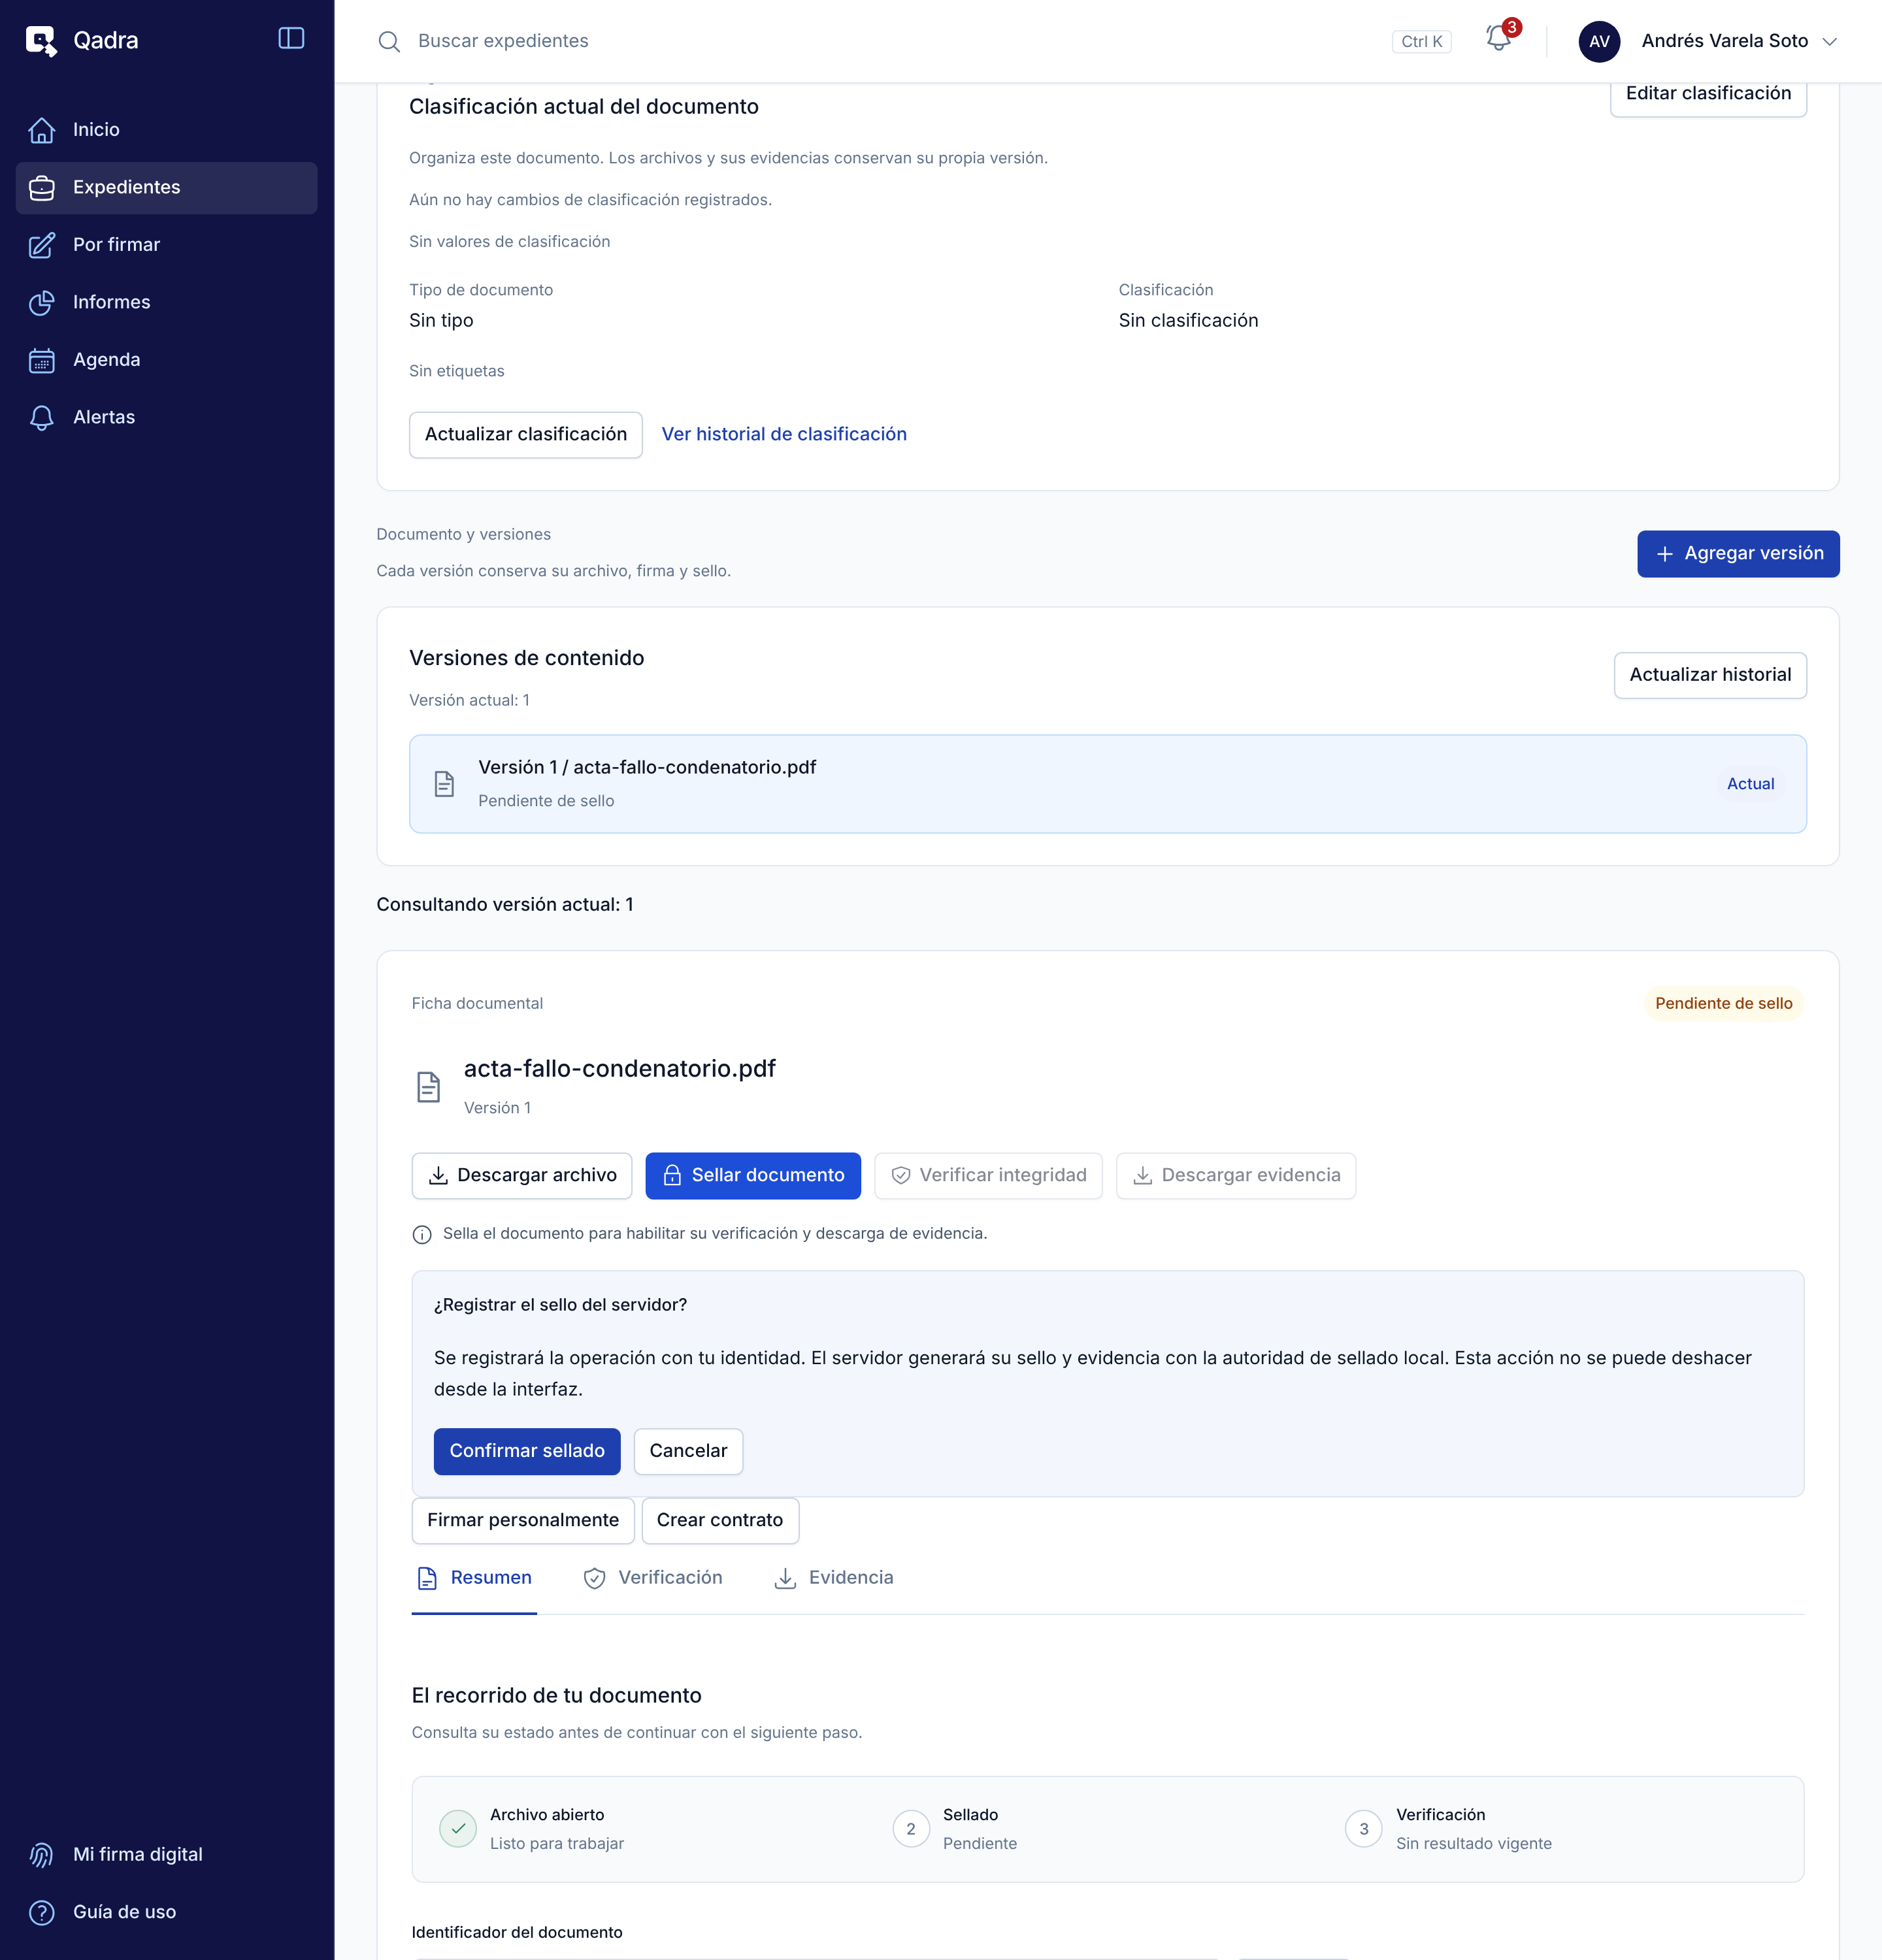
\includegraphics[width=0.9\textwidth]{capturas/A-23-sellar-documento.png}
  \caption{Confirmación del sellado.}
  \label{fig:manual-sellar-documento}
\end{figure}

\resultado Aparece \enquote{Documento sellado correctamente.} y el estado
cambia a \textbf{Sellado}.

\begin{itemize}
  \item \textbf{Resultado incierto:} si se pierde la conexión, aparece
        \enquote{El resultado del sellado es incierto. Consulta esta versión
        antes de otra decisión.} Haga clic en
        \textbf{Consultar estado del sellado}. Selle de nuevo solo si
        aparece \enquote{Esta versión sigue sin sello. Puedes iniciar una
        nueva confirmación.}
  \item El Asistente legal ve \enquote{Solicita al administrador o a un
        litigante que selle el documento para verificarlo o descargar su
        evidencia.}
\end{itemize}

% ---------------------------------------------------------------------
\section{Verificar un documento}\label{sec:verificar-documento}

\paraque Comprueba que el archivo sellado no cambió y que su firma, su
certificado y su sello de tiempo son correctos.

\disponible Administrador, Litigante y Asistente legal. La versión debe
estar sellada.

\pasos
\begin{enumerate}
  \item En la ficha del documento, haga clic en
        \textbf{Verificar integridad}.
  \item Abra la pestaña \textbf{Verificación} y revise el
        \textbf{Resultado de verificación}.
\end{enumerate}

\begin{figure}[H]
  \centering
  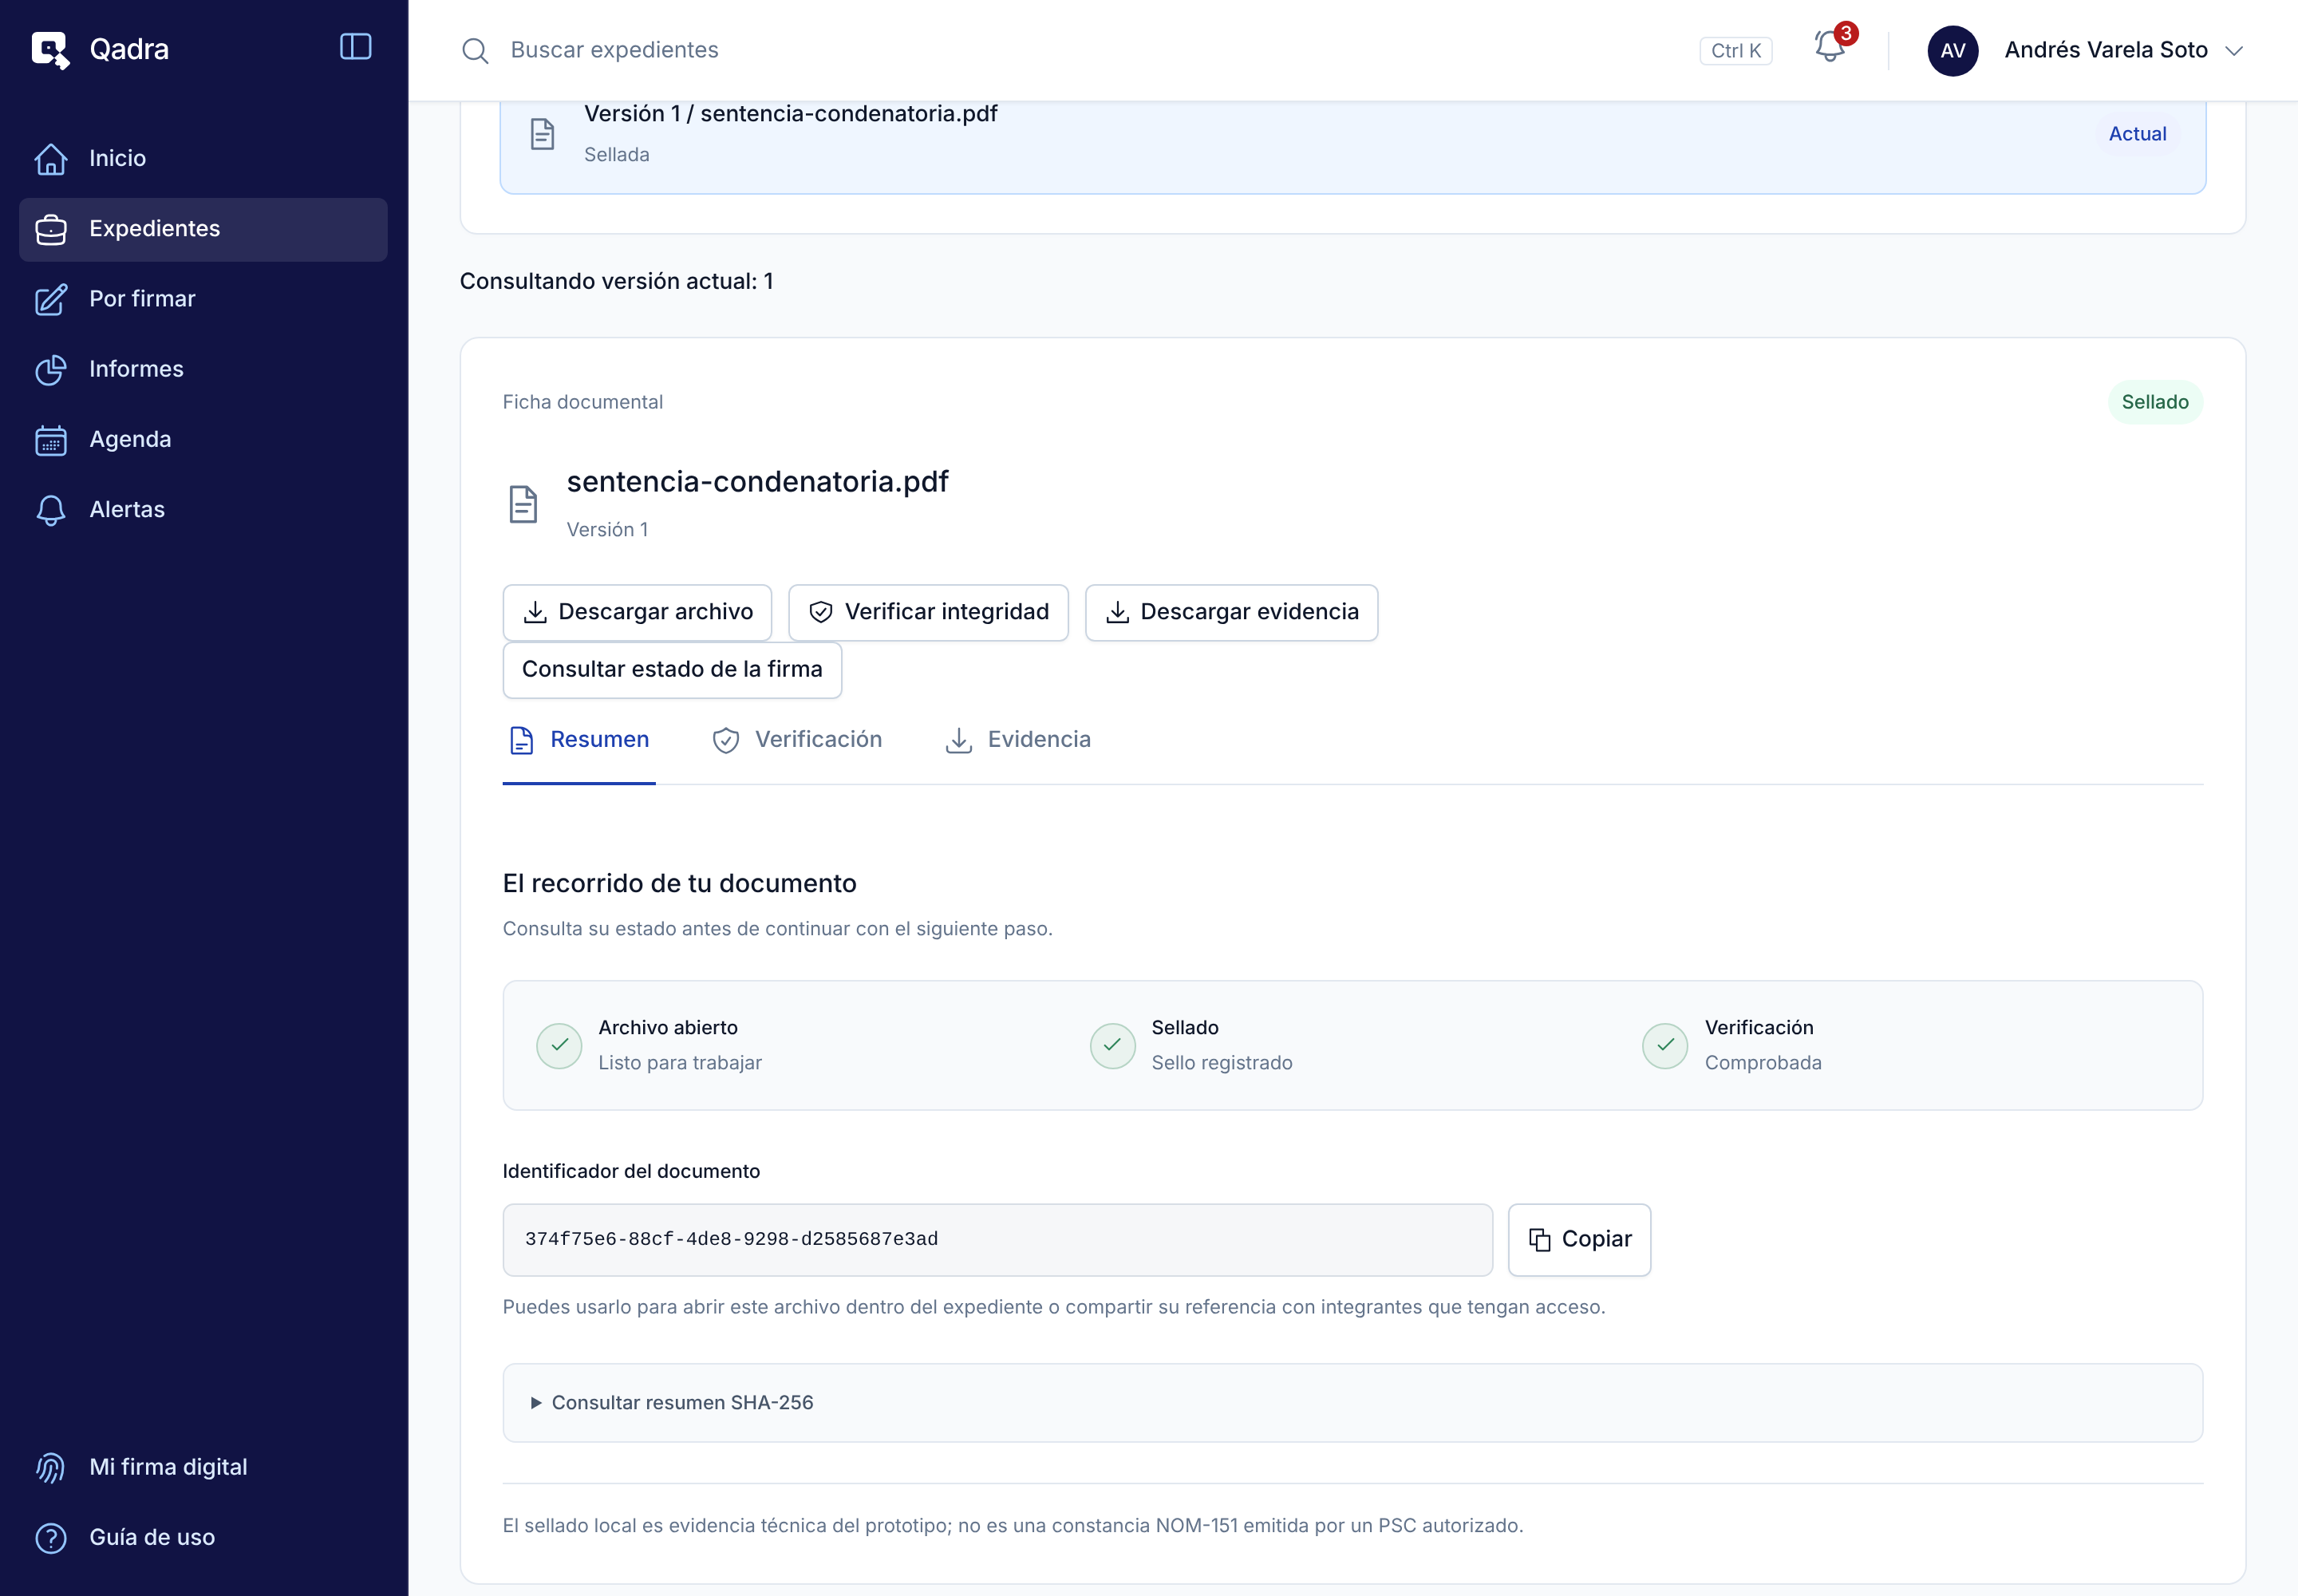
\includegraphics[width=0.9\textwidth]{capturas/A-24-resultado-verificacion.png}
  \caption{Resultado de la verificación.}
  \label{fig:manual-resultado-verificacion}
\end{figure}

\resultado Aparece \textbf{Verificación válida} con las cuatro
comprobaciones en \textbf{Correcto}.

\begin{table}[H]
  \centering
  \caption{Comprobaciones de la verificación.}\label{tab:comprobaciones}
  \begin{tabularx}{\textwidth}{L{4.2cm} Y}
    \toprule
    \textbf{Comprobación} & \textbf{Cuando está \textbf{Correcto}} \\
    \midrule
    \textbf{Integridad del archivo}    & El archivo no cambió desde que se selló. \\
    \textbf{Firma digital}             & La firma corresponde al archivo. \\
    \textbf{Certificado y revocación}  & El certificado es válido y no está revocado. \\
    \textbf{Sello de tiempo}           & El sello de tiempo corresponde al archivo. \\
    \bottomrule
  \end{tabularx}
\end{table}

\importante{Si alguna comprobación muestra \textbf{Revisar}, el resultado es
\textbf{Verificación no válida} y el documento aparece como
\textbf{Revisar evidencia}. No use esa evidencia: avise al Administrador y
consulte \textbf{Ver detalles técnicos de la verificación}.}

% ---------------------------------------------------------------------
\section{Descargar y validar la evidencia}\label{sec:descargar-evidencia}

\paraque Descarga un paquete ZIP con el documento y todo lo necesario para
comprobarlo fuera de Qadra.

\disponible Administrador, Litigante y Asistente legal. La versión debe
estar sellada.

\pasos
\begin{enumerate}
  \item En la ficha del documento, haga clic en
        \textbf{Descargar evidencia}.
  \item Guarde el archivo \texttt{evidencia-[identificador]-v[versión].zip}
        sin descomprimirlo ni modificarlo.
  \item Para validarlo en el navegador, abra la pestaña \textbf{Evidencia}.
        En \textbf{Validar un paquete de evidencia}, seleccione el ZIP en
        \textbf{Paquete de evidencia (ZIP)} y haga clic en
        \textbf{Validar paquete}.
\end{enumerate}

\begin{figure}[H]
  \centering
  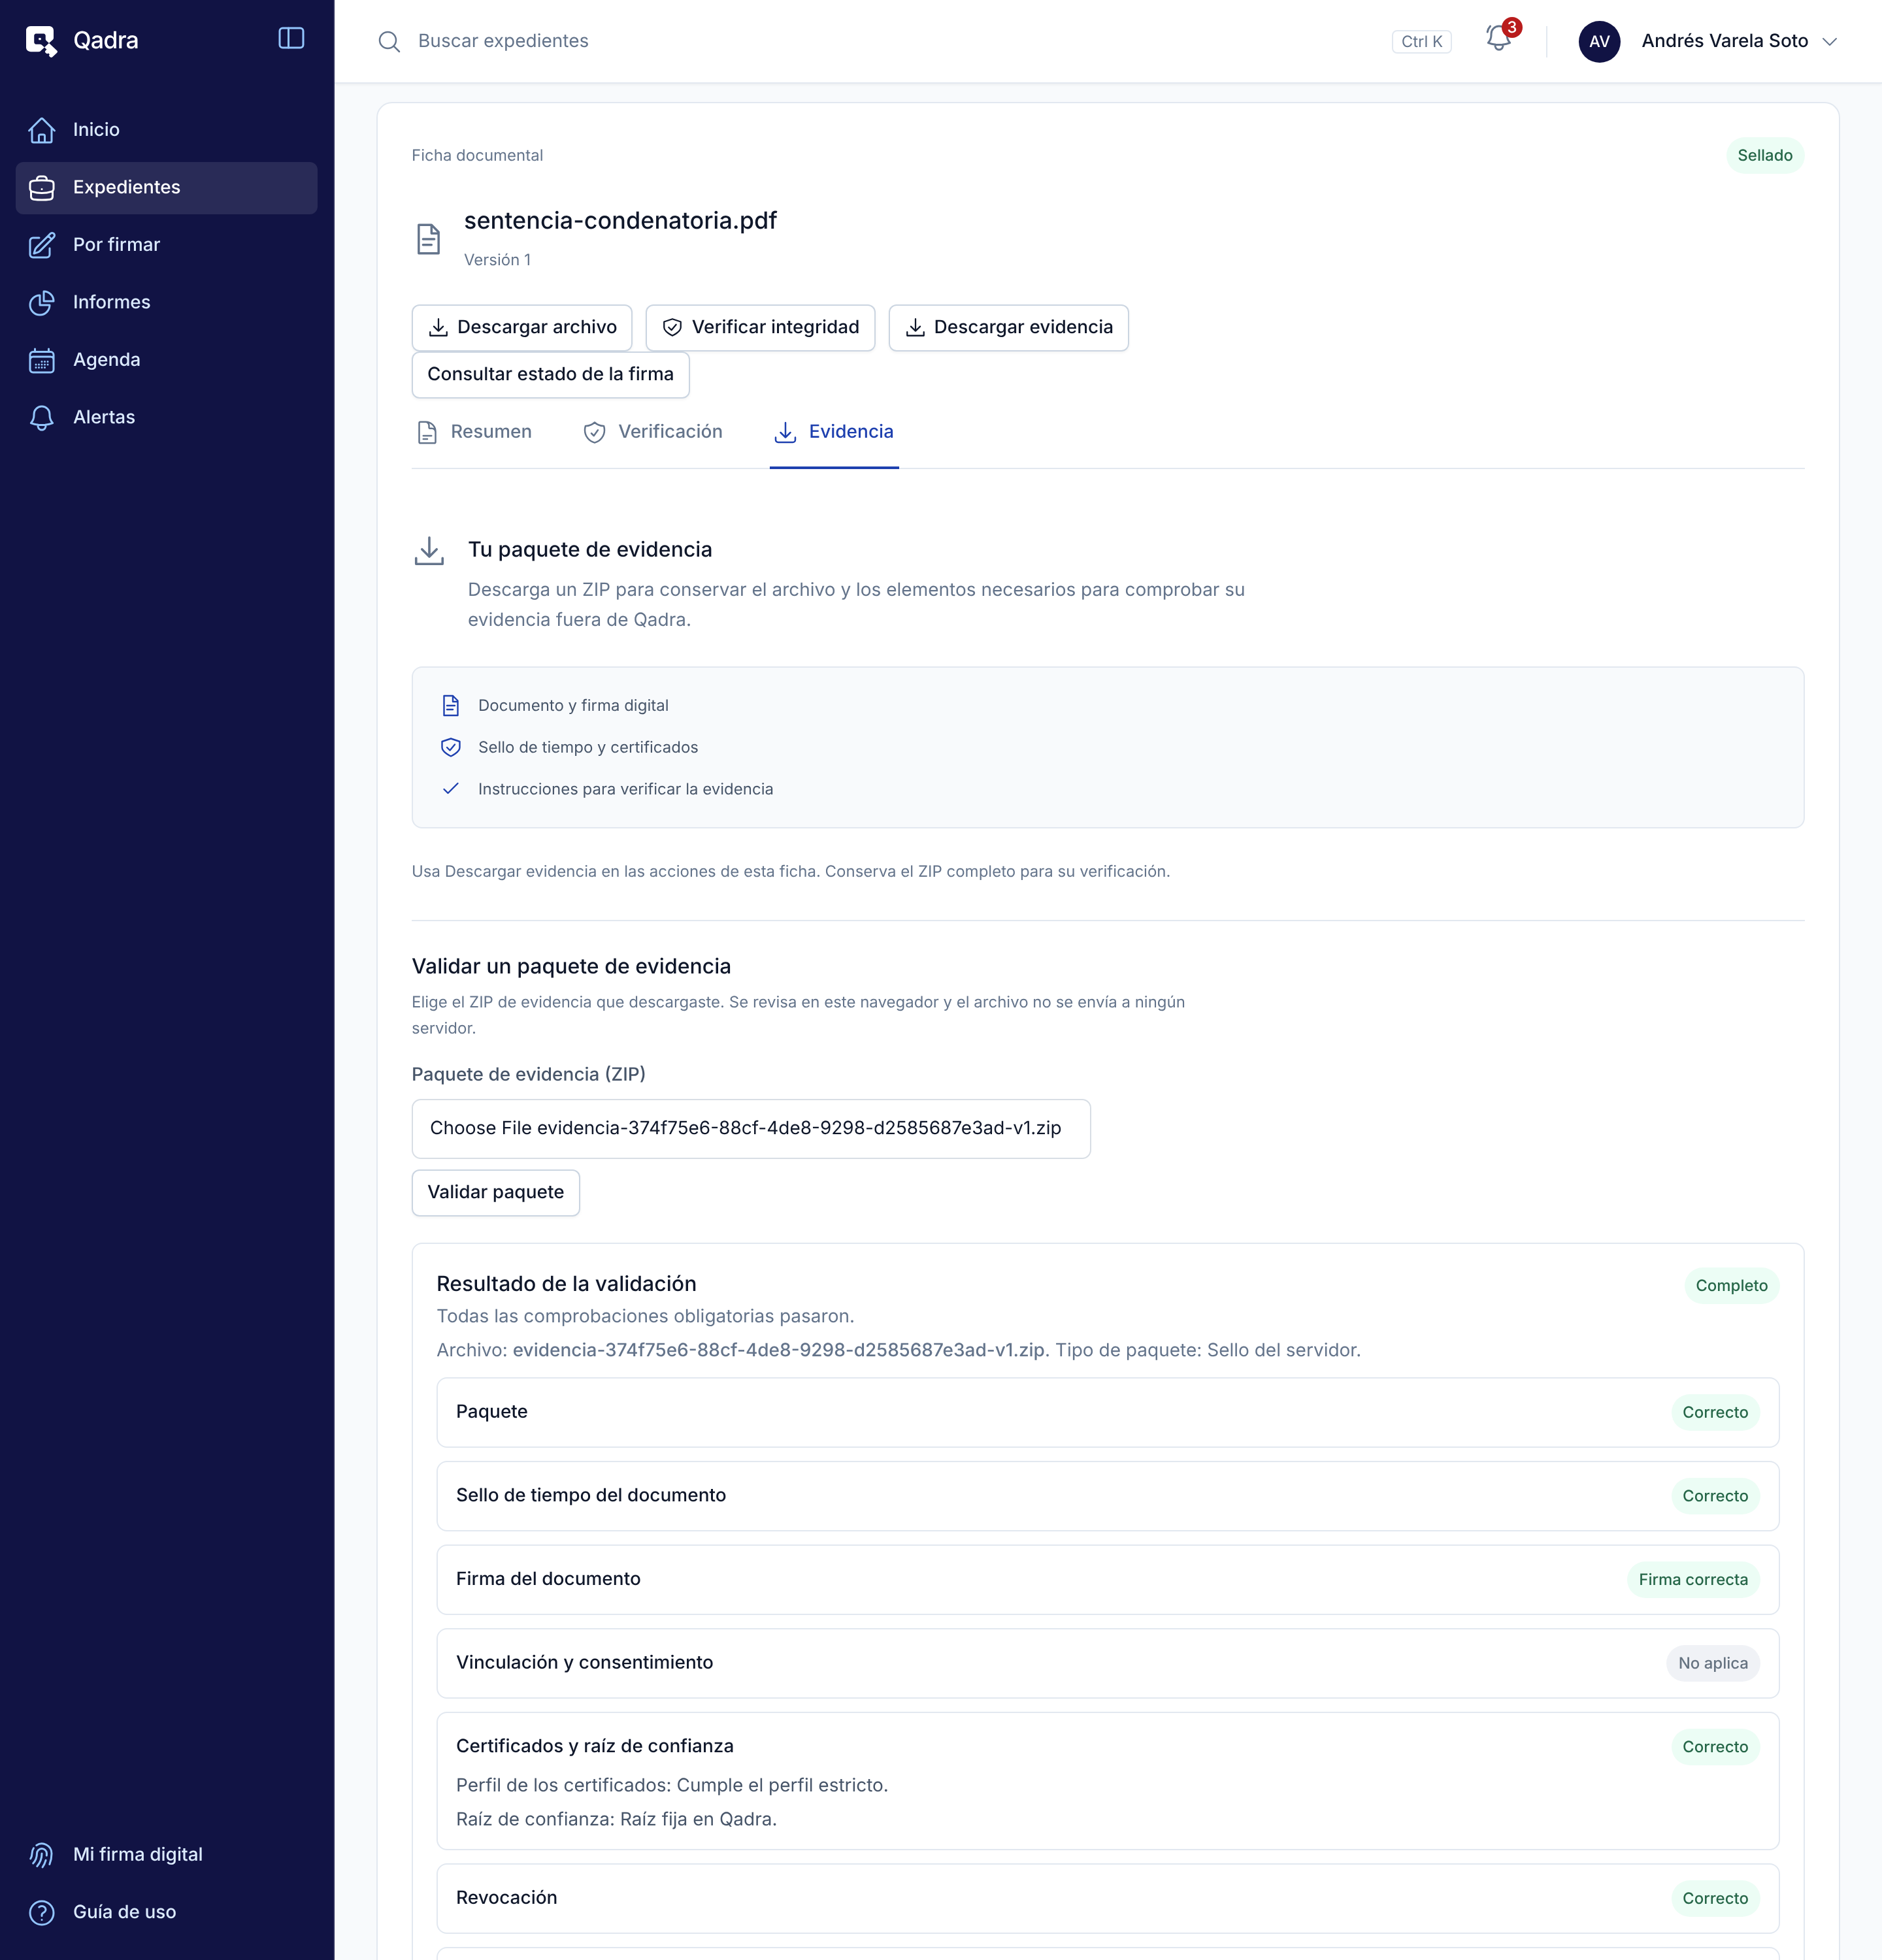
\includegraphics[width=0.9\textwidth]{capturas/A-25-evidencia.png}
  \caption{Paquete de evidencia y su validación.}
  \label{fig:manual-evidencia}
\end{figure}

\resultado Aparece \enquote{Evidencia descargada.} Al validarlo, el resultado
\textbf{Completo} indica que todas las comprobaciones obligatorias pasaron.

\begin{itemize}
  \item El paquete contiene el documento y su firma, el sello de tiempo, los
        certificados y las instrucciones para verificarlo.
  \item La validación se hace en su navegador; el archivo no se envía a
        ningún servidor.
  \item Los resultados posibles de la validación se explican en la \cref{tab:resultado-validacion}.
        Cualquier persona puede verificar el ZIP sin cuenta, siguiendo la
        verificación independiente del \cref{cap:verificacion-independiente}.
\end{itemize}

% ---------------------------------------------------------------------
\section{Firmar personalmente un documento}\label{sec:firma-personal}

\paraque Firma una versión PDF con su propio certificado, en lugar del sello
del servidor.

\disponible Litigante, con un certificado vinculado en
\textbf{Mi firma digital}. La versión debe ser PDF, no estar sellada ni en
contrato, y el expediente debe estar activo.

Tenga a la mano su clave privada cifrada (archivo \texttt{.pem}) y su
contraseña.

\pasos
\begin{enumerate}
  \item En la ficha del documento, haga clic en
        \textbf{Firmar personalmente}.
  \item Haga clic en \textbf{Revisar PDF} y lea el documento.
  \item Marque \textbf{He revisado este PDF y confirmo su contenido}.
  \item En \textbf{Firmar en este dispositivo}, seleccione su
        \textbf{Clave privada cifrada}, escriba la
        \textbf{Contraseña de la clave} y haga clic en
        \textbf{Firmar localmente}.
  \item Haga clic en \textbf{Preparar consentimiento}.
  \item Marque \textbf{Confirmo firmar esta versión con mi certificado} y
        firme de nuevo con \textbf{Firmar localmente}.
  \item Haga clic en \textbf{Enviar firma personal}.
\end{enumerate}

\begin{figure}[H]
  \centering
  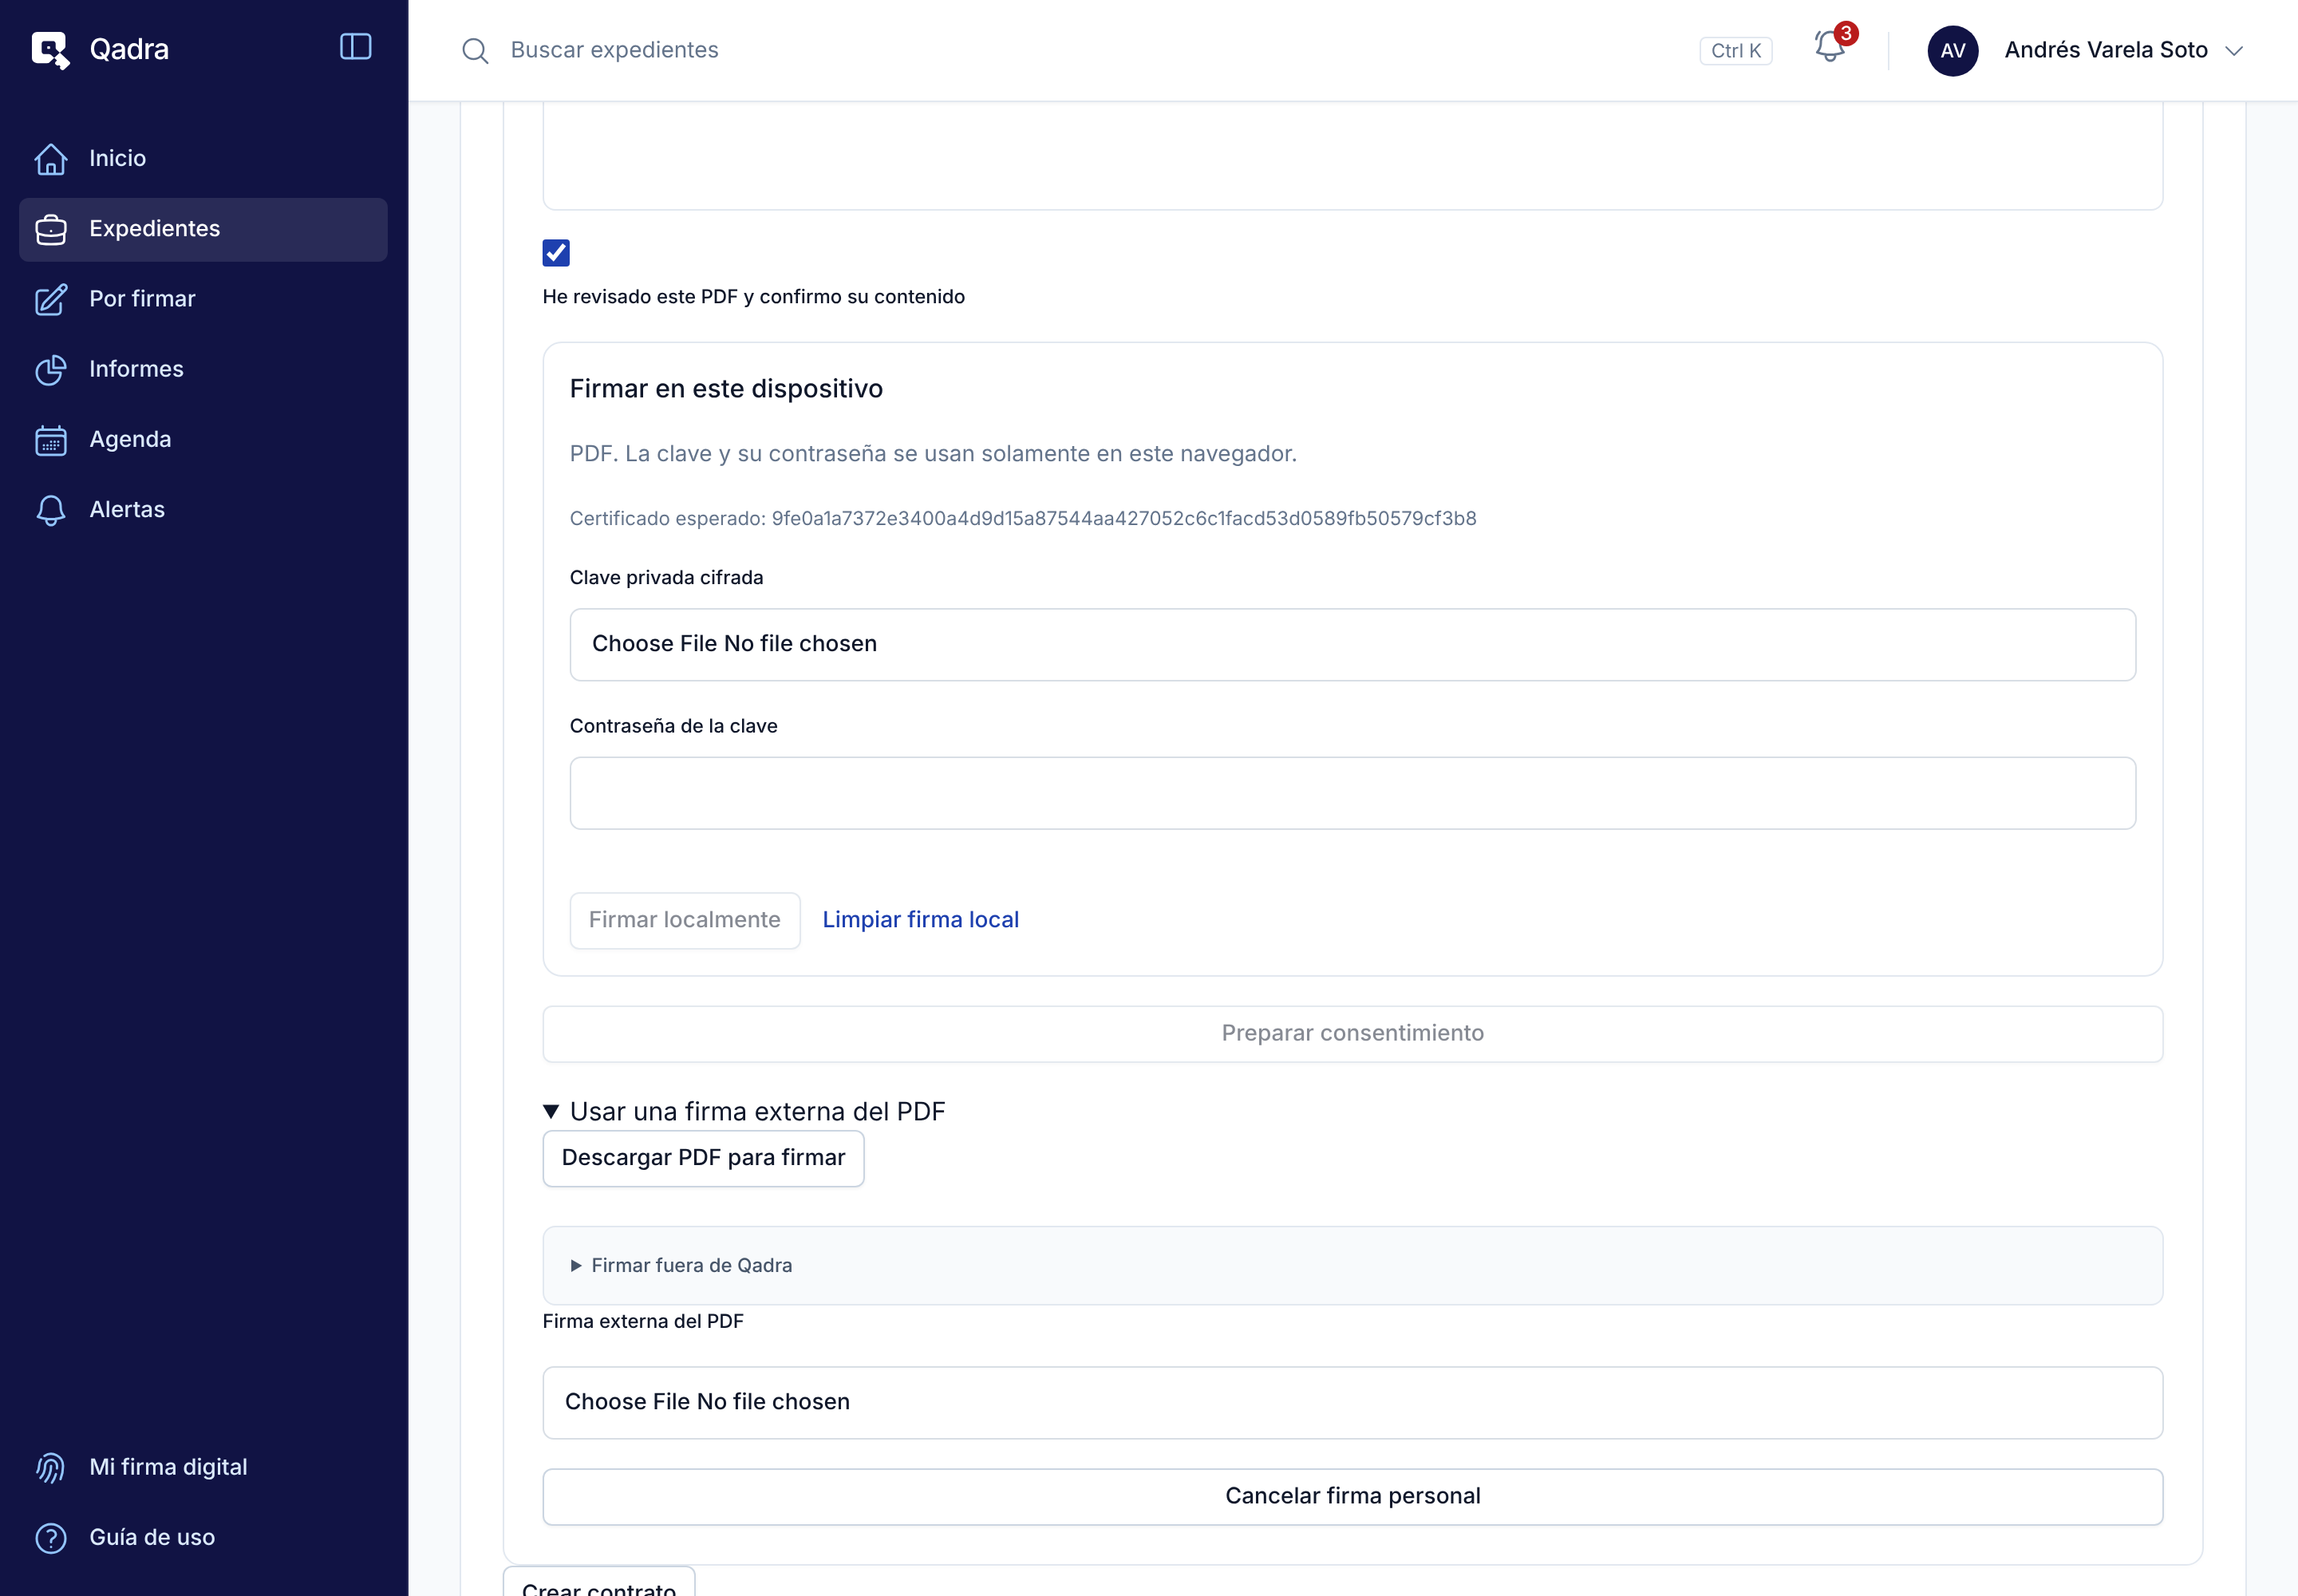
\includegraphics[width=0.9\textwidth]{capturas/A-26-firma-personal.png}
  \caption{Firma personal de un documento.}
  \label{fig:manual-firma-personal}
\end{figure}

\resultado Aparece \textbf{Firma personal aceptada} y la versión queda
\textbf{Sellado}. Haga clic en \textbf{Descargar recibo de firma} para
conservar el recibo.

\begin{itemize}
  \item Si no tiene certificado vinculado, aparece \enquote{Primero registra
        tu certificado en Mi firma digital.}
  \item Para firmar con su propia herramienta, use
        \textbf{Usar una firma externa del PDF} y
        \textbf{Usar una firma externa del consentimiento}.
  \item Si se pierde la respuesta, haga clic en
        \textbf{Consultar recibo de firma}; consultar no vuelve a enviar la
        firma.
  \item Para revisar después el resultado, haga clic en
        \textbf{Consultar estado de la firma}.
\end{itemize}
